\documentclass[11pt]{article}
\usepackage[utf8]{inputenc}
\usepackage[
	letterpaper,
	left = .5in,
	right = .5in,
	top = 1in,
	bottom  = 1in
]{geometry}
\setlength{\columnsep}{.25in}
\usepackage{graphicx}
\usepackage{mathptmx}
\usepackage{float}
\usepackage[cmex10]{amsmath}
\usepackage{amsthm,amssymb}
\usepackage{url}
\urlstyle{same} 
\def\UrlBreaks{\do\/\do-}
\usepackage{breakurl}
\usepackage{fancybox}
\usepackage{breqn}
\usepackage{array}
\usepackage{caption}
\usepackage{subcaption}
\usepackage{comment}
\usepackage[english]{babel}
\usepackage[acronym,nomain]{glossaries} % list of acronyms
\usepackage{xurl}
\usepackage{multicol}
\usepackage{multirow}
\usepackage{mathptmx}
\usepackage{float}
\usepackage{lipsum}
\usepackage{framed}
\usepackage[T1]{fontenc}
\usepackage[pdfpagelabels,pdfusetitle,colorlinks=false,pdfborder={0 0 0}]{hyperref}
\usepackage{algorithm}
\usepackage{algpseudocode}
\usepackage{tabularx}
\usepackage{wrapfig}
%\usepackage{enumitem}
\usepackage{paralist}

% draw a frame around given text
\newcommand{\framedtext}[1]{%
	\par%
	\noindent\fbox{%
		\parbox{\dimexpr\linewidth-2\fboxsep-2\fboxrule}{#1}%
	}%
}

\renewcommand{\arraystretch}{1.2}

\sloppy
\raggedbottom

\newcolumntype{C}[1]{>{\centering\let\newline\\\arraybackslash\hspace{0pt}}m{#1-2\tabcolsep}}

\usepackage[%
backend=bibtex,     % biber or bibtex
%style=authoryear,    % Alphabeticalsch
style=numeric-comp,  % numerical-compressed
sorting=none,        % no sorting
sortcites=true,      % some other example options ...
block=none,
indexing=false,
citereset=none,
isbn=true,
url=true,
doi=true,           % prints doi
natbib=true,         % if you need natbib functions
]{biblatex}
\addbibresource{./sources/sources.bib,}  % better than \bibliography

\title{Impact of EVSE Deployment on Electrified Road Transportation Access for Long Trips}
\author{Aaron I. Rabinowitz, Vaishnavi Karanam, Radhika Gupta, others (Gil Tal?, Alan Jenn?, Susan Handy? Yue Yue Fan?)}
\date{}

\newacronym{ghg}{GHG}{Green-House Gas}
\newacronym{fe}{FE}{Fuel Economy}
\newacronym{ee}{EE}{Energy Economy}
\newacronym{epa}{EPA}{Environmental Protection Agency}
\newacronym{oem}{OEM}{Original Equipment Manufacturer}
\newacronym{ice}{ICE}{Internal Combustion Engine}
\newacronym{icv}{ICV}{Internal Combustion Vehicle}
\newacronym{icev}{ICEV}{Internal Combustion Engine Vehicle}
\newacronym{em}{EM}{Electric Motor}
\newacronym{hev}{HEV}{Hybrid Electric Vehicle}
\newacronym{ev}{EV}{Electric Vehicle}
\newacronym{phev}{PHEV}{Plug-in Hybrid Electric Vehicle}
\newacronym{lrphev}{LR-PHEV}{Long Range PHEV}
\newacronym{srphev}{SR-PHEV}{Short Range PHEV}
\newacronym{mhev}{MHEV}{Mild Hybrid Electric Vehicle}
\newacronym{pev}{PEV}{Plug-in Electric Vehicle}
\newacronym{bev}{BEV}{Battery Electric Vehicle}
\newacronym{cbev}{CBEV}{City BEV}
\newacronym{afv}{AFV}{Alternative Fuel Vehicle}
\newacronym{fcev}{FCEV}{Fuel Cell Electric Vehicle}
\newacronym{cav}{CAV}{Connected Autonomous Vehicle}
\newacronym{fc}{FC}{Fuel Consumption}
\newacronym{ec}{EC}{Energy Consumption}
\newacronym{dtto}{DTTO}{Discrete Time Trajectory Optimization}
\newacronym{udto}{UDTO}{Uniformly Discretized Trajectory Optimization}
\newacronym{sto}{STO}{Spline Trajectory Optimization}
\newacronym{rbed}{RBED}{Rules-Based Eco-Driving}
\newacronym{cidm}{CIDM}{Cooperative Intelligent Driver Model}
\newacronym{idm}{IDM}{Intelligent Driver Model}
\newacronym{soc}{SOC}{State of Charge}
\newacronym{ocp}{OCP}{Optimal Control Problem}
\newacronym{ttc}{TTC}{Time-To-Collision}
\newacronym{dp}{DP}{Dynamic Programming}
\newacronym{ga}{GA}{Genetic Algorithm}
\newacronym{sdm}{SDM}{Smart Driver Model}
\newacronym{v2i}{V2I}{Vehicle to Infrastructure}
\newacronym{v2v}{V2V}{Vehicle to Vehicle}
\newacronym{v2x}{V2X}{Vehicle to Everything}
\newacronym{hil}{HIL}{Hardware In Loop}
\newacronym{pso}{PSO}{Particle Swarm Optimization}
\newacronym{dt}{DT}{Direct Transcription}
\newacronym{oedt}{OEDT}{Optimal Eco-Driving Trace}
\newacronym{fods}{FODS}{Forward Object Detection System}
\newacronym{cas}{CAS}{Collision Aviodance System}
\newacronym{acc}{ACC}{Adaptive Cruise Control}
\newacronym{obu}{OBU}{On-Board Unit}
\newacronym{rsu}{RSU}{Road-Side Unit}
\newacronym{sae}{SAE}{Society of Automotive Engineers}
\newacronym{adas}{ADAS}{Advanced Driver Assistance System}
\newacronym{edc}{EDC}{Eco-Driving Control}
\newacronym{lv}{LV}{Lead Vehicle}
\newacronym{ss}{SS}{Segment Speeds}
\newacronym{hs}{HS}{Historical Speeds}
\newacronym{spat}{SPAT}{Signal Phase and Timing}
\newacronym{map}{MAP}{Positions of Subsequent Traffic Lights}
\newacronym{al2n}{AL2N}{Acceleration L\textsuperscript{2} Norm}
\newacronym{rpc}{RPC}{Road Power Cost}
\newacronym{bpc}{BPC}{Battery Power Cost}
\newacronym{fecc}{FECC}{Fitted Equivalent Consumption Cost}
\newacronym{ipopt}{IPOPT}{Interior-Point Optimization}
\newacronym{dtnlp}{DTNLP}{Discreet-Time Non-Linear Programming}
\newacronym{snlp}{SNLP}{Spline Non-Linear Programming}
\newacronym{sga}{SGA}{Spline Genetic Algorithm}
\newacronym{spso}{SPSO}{Spline Particle Swarm Optimization}
\newacronym{2sdp}{2SDP}{2 State Dynamic Programming}
\newacronym{aos}{AOS}{Approximate Optimal Spline}
\newacronym{pchip}{PCHIP}{Piecewise Cubic Hermitic Interpolation Polynomial}
\newacronym{nrel}{NREL}{National Renewable Energy Laboratory}
\newacronym{fastsim}{FASTSim}{Future Automotive Systems Technology Simulator}
\newacronym{mfei}{MFEI}{Mean Fuel Economy Improvement}
\newacronym{pas}{PAS}{Percent Acceptable Solutions}
\newacronym{mrt}{MRT}{Mean Run-Time}
\newacronym{mpc}{MPC}{Model Predictive Control}
\newacronym{adp}{ADP}{Approximate Dynamic Programming}
\newacronym{rl}{RL}{Reinforcement Learning}
\newacronym{mbrl}{MBRL}{Model Based Reinforcement Learning}
\newacronym{nlp}{NLP}{Non-Linear Programming}
\newacronym{nhtsa}{NHTSA}{National Highway Traffic Safety Administration}
\newacronym{aeb}{AEB}{Automatic Emergency Braking}
\newacronym{tsdc}{TSDC}{Transportation Secure Data Center}
\newacronym{anl}{ANL}{Argonne National Lab}
\newacronym{d3}{D\textsuperscript{3}}{Downloadable Dynamometer Database}
\newacronym{cd}{C\textsubscript{D}}{Coefficient of Drag}
\newacronym{crr}{C\textsubscript{RR}}{Coefficient of Rolling Resistance}
\newacronym{mape}{MAPE}{Mean Absolute Percentage Error}
\newacronym{evse}{EVSE}{Electric Vehicle Supply Equipment}
\newacronym{ld}{LD}{Light Duty}
\newacronym{md}{MD}{Medium Duty}
\newacronym{hd}{HD}{Heavy Duty}
\newacronym{mdhd}{MD/HD}{Medium Duty / Heavy Duty}
\newacronym{inrix}{INRIX}{}
\newacronym{epri}{EPRI}{Electric Power Research Institute}
\newacronym{nhts}{NHTS}{National Highway Transportation Survey}
\newacronym{usa}{USA}{United States of America}
\newacronym{sof}{SOF}{State of Fuel}
\newacronym{hc}{HC}{Home Charging}
\newacronym{bc}{BC}{Battery Capacity}
\newacronym{dcl}{DCL}{Destination Charger Likelihood}
\newacronym{ercr}{ERCR}{En-Route Charging Rate}
\newacronym{ercp}{ERCP}{En-Route Charging Penalty}
\newacronym{ftc}{FTC}{Fuel Tank Capacity}
\newacronym{ftp}{FTP}{Fuling Time Penalty}
\newacronym{psrc}{PSRC}{Puget Sound Regional Council}
\newacronym{bts}{BTS}{Bureau of Transportation Statistics}
\newacronym{happ}{HAPP}{Household Activity Pattern Problem}
\newacronym{chts}{CHTS}{California Houslehold Travel Survey}
\newacronym{dcfc}{DCFC}{DC Fast Charging}
\newacronym{liion}{Li-Ion}{Lithium-Ion}
\newacronym{lvl2}{LVL 2}{DC Level 2}
\newacronym{oems}{OEMS}{Optimal Energy Management Strategies}
\newacronym{poems}{POEMS}{Predictive Optimal Energy Management Strategies}
\newacronym{vpoems}{VP-OEMS}{Velocity Prediction enabled Optimal Energy Management Strategies}
\newacronym{gnss}{GNSS}{Global Navigational Satellite System}
\newacronym{obd2}{OBD-II}{On-Board Diagnostics II}
\newacronym{csu}{CSU}{Colorado State University}
\newacronym{wes}{WES}{Weight Efficiency Score}
\newacronym{gvwr}{GVWR}{Gross Vehicle Weight Rating}
\newacronym{fha}{FHA}{Federal Highway Administration}
\newacronym{vius}{VIUS}{Vehicle Inventory and Use Survey}
\newacronym{eod}{EOD}{End of Day}
\newacronym{osrm}{OSRM}{Open-Source Routing Machine}
\newacronym{vrp}{VRP}{Vehicle Routing Problem}
\newacronym{evrp}{EVRP}{Electric Vehicle Routing Problem}
\newacronym{tsp}{TSP}{Traveling Salesman Problem}
\newacronym{can}{CAN}{Controller Area Network}
\newacronym{lstm}{LSTM}{Long Short-Term Memory}
\newacronym{ann}{ANN}{Artificial Neural Network}
\newacronym{ml}{ML}{Machine Learning}
\newacronym{fcdp}{FC-DP}{Full Cycle Dynamic Programming}
\newacronym{ppmpc}{PP-MPC}{Perfect Prediction Model Predictive Control}
\newacronym{rpmpc}{RP-MPC}{Real Prediction Model Predictive Control}
\newacronym{cvmpc}{CV-MPC}{Constant Velocity Model Predictive Control}
\newacronym{mae}{MAE}{Mean Absolute Error}
\newacronym{fsmvrp}{FSMVRP}{Fleet Size and Mix Vehicle Routing Problem}
\newacronym{mcvrp}{MCVRP}{Monte-Carlo Vehicle Routing Problem}
\newacronym{ppf}{PPF}{Percent Point Function}
\newacronym{ccdng}{CCDNG}{Completely Connected Directional Network Graph}
\newacronym{sho}{SHO}{Spline Heuristic-Optimal}
\newacronym{npv}{NPV}{Net Present Value}
\newacronym{tco}{TCO}{Total Cost of Ownership}
\newacronym{mtk}{MTK}{Metric-Ton-Kilometer}
\newacronym{lco}{LCO}{Levelized Cost of Ownership}
\newacronym{lcod}{LCOD}{Levelized Cost of Driving}
\newacronym{sme}{SME}{Subject Matter Expert}
\newacronym{doe}{DOE}{Deparment of Energy}
\newacronym{vmt}{VMT}{Vehicle Miles Traveled}
\newacronym{dot}{DOT}{Department of Transportation}
\newacronym{ltl}{LTL}{Less Than Truckload}
\newacronym{lpcp}{LPCP}{Lost Payload Capacity Portion}
\newacronym{chaas}{ChaaS}{Charging as a Service}
\newacronym{tou}{TOU}{Time of Use}
\newacronym{ocs}{OCS}{Optimal Charging Strategy}
\newacronym{soe}{SOE}{State of Energy}
\newacronym{ltp}{LTP}{Lost Time Portion}
\newacronym{yd}{YD}{Yearly Distance}
\newacronym{dd}{DD}{Daily Distance}
\newacronym{vnr}{VNR}{Vehicle Nominal Range}
\newacronym{nyo}{NYO}{Number of Years of Ownership}
\newacronym{ap}{AP}{Age at Purchase}
\newacronym{dpm}{DPM}{Diesel Price Multiplier}
\newacronym{epm}{EPM}{Electricity Price Multiplier}
\newacronym{evsep}{EVSEP}{EVSE Premium}
\newacronym{pe}{PE}{Payload Exemption}
\newacronym{bpp}{BPP}{Battery Pack Pricing}
\newacronym{my}{MY}{Model Year}
\newacronym{ipfn}{IPFN}{Iterative Proportional Fitting with N dimensions}
\newacronym{dco}{DCO}{Discretized Control Optimization}
\newacronym{pto}{PTO}{Polynomial Trajectory Optimization}
\newacronym{slsqp}{SLSQP}{Sequential Least Squares Programming}
\newacronym{aer}{AER}{All Electric Range}
\newacronym{msrp}{MSRP}{Manufacturer Recommended Sales Price}
\newacronym{afdc}{AFDC}{Alternative Fuels Data Center}
\newacronym{uf}{UF}{Utility Factor}
\newacronym{hov}{HOV}{Hich Occupancy Vehicle}
\newacronym{lp}{LP}{Linear Problem}
\newacronym{qp}{QP}{Quadratic Problem}
\newacronym{sp}{SP}{Stochastic Problem}
\newacronym{slp}{S-LP}{Stochastic Linear Problem}
\newacronym{milp}{MILP}{Mixed Integer Linear Problem}
\newacronym{smilp}{S-MILP}{Stochastic Mixed Integer Linear Problem}
\newacronym{los}{LOS}{Level of Service}
\newacronym{v2s}{V2S}{Vehicle-to-Structure}
\newacronym{v2g}{V2G}{Vehicle-to-Grid}
\newacronym{gacm}{GACM}{Grid-Aware Charge Management}
\newacronym{iso}{ISO}{Independent System Operator}
\newacronym{dcopf}{DC-OPF}{DC Optimal Power Flow}
\newacronym{lmp}{LMP}{Location Marginal Price}
\newacronym{gcc}{GCC}{Giant Connected Component}
\newacronym{hjb}{HJB}{Hamilton-Jacobi-Bellman}
\newacronym{pdf}{PDF}{Probability Distribution Function}
\newacronym{scram}{SCRAM}{Stochastic Cost with Risk Allowance Minimization}
\newacronym{scramd}{SCRAM-D}{SCRAM-Dijkstra}
\newacronym{scramb}{SCRAM-B}{SCRAM-Bellman}
\newacronym{rsic}{RSIC}{Range-Sensitive Information Centrality}
\newacronym{rsbc}{RSBC}{Range-Sensitive Betweenness Centrality}
\newacronym{ras}{RAS}{Range Addition Station}

\makeglossaries

\begin{document}

\maketitle

\section*{Abstract}

A well designed transportation system provides sufficient access from origins to destinations to accommodate household and business demand in an economy.  Increasingly, climate action goals require that more transportation load be shifted to less \gls{ghg} intensive modes among which are \glspl{bev}. While \glspl{bev} use the same roads as \glspl{icev} they draw energy from a separate network of stations which neither as robust as nor coincident to the \gls{icev} fueling network, a consequence of the different current and historical economics of both. Insufficiency and unreliability of public DC \gls{evse} which is primarily used for charging on long itineraries mean that \gls{bev} drivers, depending on vehicle range and risk attitude, may opt for less direct paths with lower charging risk, opt for a more \gls{ghg} intensive mode, or abandon an itinerary. Holistically, the transportation system provides less access to \glspl{bev} for distant pairs. This project develops methods and tools to optimize deployment of future \gls{evse} to mitigate the issue. Methods herein are based on range and charging risk sensitive optimal routing between O/D pairs subject to the locations and usability rates of \gls{evse}. These methods and tools may be used by policy makers to directly evaluate the impact of proposed stations on \gls{bev} transportation access.
\medskip

\begin{multicols}{2}

\section*{Introduction}

Developed economies rely on their transportation sectors to move persons and goods in astounding volumes underpinning multi-trillion dollar yearly outputs and setting the conditions for households and individuals. The concept of transportation access can roughly be considered as the inverse of the difficulty of reaching selected destinations from selected origins. More efficient transportation allows for individuals and businesses to access more opportunities for the same expenditure in time and/or money. Transportation access is, thus, a nuanced and multi-dimensional concept which must vary, at least, by location, entity, and scope. Further complexity is added by the reality that all elements of the global transportation system are, to a greater or lesser degree, connected. How one selects \gls{od} pairs and the entities which must transit them will color one's analysis. It is, thus, important to carefully define the scope of analysis.

Transportation researchers and planners have introduced the concept of transportation accessibility primarily as it applies to routine household behavior. From the personal transportation perspective, access is defined as the ease with which individuals can reach the destinations they need or desire, considering both the distribution of destinations and the various transportation options available \cite{Handy_2020}. Accessibility is influenced by several key factors. Land-use dynamics determine the distribution and demand for amenities like jobs and services across different locations, while transportation factors such as travel time, costs, and infrastructure availability also play a significant role \cite{Geurs_2004}. Temporal considerations reflect the availability of opportunities throughout the day, and individual characteristics such as age, income, and education predict access to transportation modes and opportunities \cite{Miller_2018}.

The access provided by a road transportation system for \glspl{bev} is different than that for \glspl{icev} due to vehicular and supply network characteristics as well as individual and household characteristics. Modern \glspl{bev} possess sufficient practical ranges to accomplish much daily travel [SOURCE - or maybe derive this from NHTS]. However, for long itineraries \glspl{icev} offer greater accessibility compared to \glspl{bev} due to the extensive availability of fueling stations in contrast to charging stations. Fueling stations are widely distributed across urban, suburban, and rural areas, ensuring that drivers have convenient access to refueling points wherever they travel. In contrast, the \gls{evse} network is less developed and distributed. This infrastructure gap poses challenges for \gls{bev} drivers, especially in remote or less densely populated areas, leading to concerns about range anxiety and limitations on travel options. Inadequate access for \gls{bev} may result in trip cancellations or mode switches, often favoring \gls{icev} or air travel.

While incentives for \gls{evse} deployment can help mitigate this issue, it may not fully resolve the disparities which result from the different economic models. Gas pumping equipment requires lower up-front costs than DC \gls{evse} and is cheaper to operate \cite{Gamage_2023}. It is, nevertheless, the case that gas is often sold at low markup or a slight loss with stations making most profit on convenience items [SOURCE]. Nearly all light-duty \gls{icev} drivers source all of their fuel from public fueling stations regardless of travel behavior [SOURCE]. \gls{bev} drivers are expected to, and currently do, source much of their electricity from AC supply equipment during long dwells, often at private chargers \cite{Hardman_2018}. Thus DC \gls{evse} is subject to higher capital expenditure and lower revenue potential while simultaneously benefiting less from historical investment. Public investments in EV supply infrastructure, thus, must be made judiciously. Evaluation methods for potential charging stations should consider their network-wide impact on accessibility, considering vehicle types, charging outcomes, and driver risk attitudes.

This study introduces a novel methodology to assess the impacts of vehicle electrification on the accessibility of road transportation systems subject to supply networks. The methodology will measure \gls{icev} and \gls{bev} accessibility by computing optimal-feasible travel routes of \gls{od} pairs using a Monte-Carlo Dijkstra routing algorithm subject to vehicle range limitations, infrastructure constraints and driver risk attitudes. Additionally, a case study is presented for the state of California showing a comparison between \glspl{icev} and \glspl{bev} access for important \gls{od} pairs. The methodology introduced, as well as the open-source code provided in the supplemental information will be an invaluable tool for planners and policymakers in originating and evaluating \gls{evse} deployment policies.

\section*{Transportation Accessibility}

Transportation access has been studied as a tool for urban and regional planners since the middle of the 20\textsuperscript{th} century with theoretical origins in the theory of population migration proposed by Ravenstein in 1885 \cite{Ravenstein_1885}. The movement of people over a given time-scale can be analogized to an electrical circuit. In this analogy push and pull factors determine are the "voltage" separation, traversal difficulty is the "resistance" and the resulting flow is the "current". The field of transportation accessibility uses this framework to study the efficiency of a region. The accepted definition of transportation access is the ease with which individuals can access opportunities subject to the transportation system in the relevant area. Thus, accessibility is a framework which encompasses voltage factors such as land use and temporal availability, resistance factors such as transportation system design, and universal factors such as personal preference \cite{Geurs_2004}. Literature provides four essential frameworks for computing access as surveyed in \cite{Handy_1997, Kwan_1998, Geurs_2004, Miller_2018, Handy_2020} and discussed below.

It is not necessarily apparent what voltages occur where in a region. Individuals are assumed to need or desire location specified opportunities such as grocery shopping. However, there may be several near-equivalents for a given opportunity type. The simplest methods for quantifying voltage are based on proximity to an opportunity type \cite{Wachs_1973, Vickerman_1974}. Proximity methods consider that a person has a level of access to a given need determined by that person's proximity to the closest equivalent opportunity. These methods do not account for heterogeneity within an opportunity category nor for the benefits of redundancy within an opportunity category. The inverse are isocost methods wherein a person is said to have access to determined by the number of opportunities available within a given isocost polygon. This method has the drawback of not considering the differences in traversal cost for \gls{od} pairs within the iso-cost region. These methods have been used widely \cite{Easa_1993} due to their computational lightness and form the basis for modern big-data methods such as th US DOE's Mobility Energy Productivity metric \cite{Hou_2019}.

Proximity and isocost methods are easy to compute because they treat redundancy arbitrarily respectively by neglecting it and by defining a region of consideration. Equivalent and near-equivalent opportunities compete with one-another if sufficiently proximate or if the paths required to reach them overlap \cite{Stouffer_1940}. Gravity/entropy methods \cite{Noulas_2012, Jung_2008} address this shortcoming. These methods are so called as they concern the cumulative effect of opportunities for a given origin on the basis of demand over proximity (gravity) or information content (entropy). Such methods were first formalized into a quantitative framework in 1959 \cite{Hansen_1959} as a generalization of previous methodology for quantifying the efficiency of urban land use. Gravity/entropy methods define accessibility as the intensity of the possibility for interaction thus focusing on the voltage separation (demand for opportunities) and the resistance (difficulty of traversal for \gls{od} pairs). Gravity/entropy methods consider the cumulative effect of equivalent opportunities at different locations for each origin with their impact weighed by their proximity. Implicit in the formulation of gravity/entropy methods is that every opportunity has some effect on every individual even if this is, often, negligible and the effect of any one opportunity is determined by its individual proximity and those of all others.

Proximity and gravity/entropy methods rely on the assumption that traversal cost is the primary factor determining individuals decision to select one opportunity from among a set of similar entities. While this is certainly true if the difference in traversal cost is large enough it is not, altogether, obvious what the threshold of disambiguation is or if this is similar among the population. Thus, researchers have proposed to use Discreet Choice Modeling \cite{Ben_Akiva_1985} to explain revealed choices wherein ease-of-access is one of several possible factors in determining the utility of a given opportunity for an individual \cite{Cevero_1995, Shen_1998, Karst_2003}.

There are, thus, a variety of methods which can be used to quantify the accessibility of a given region with varying computational and data requirements. The relationship between land-use, transportation, and demography is circular rather than linear. Which method one chooses for an analysis reflects the scope and purpose of that analysis. Definition of scope can be difficult and can lead to self-defeating policies \cite{Handy_1996}. This study is concerned with the effects of electrification on accessibility for users of road vehicles. This very specific scope neglects to specify the demand element. Rather, for a given set of demand locations, the methodology introduced quantifies the difference in access for a driver by vehicle powertrain type as a function of the vehicle and the supply network. This paper is focused on regional travel rather than local travel as this is where public DC \gls{evse} infrastructure becomes important but, it should be noted, that the method is valid for all travel scales. Methodology is developed in the following section.

\section*{Methods}

\subsection*{Vehicle Reduced Sub-Network Graph}

Critical to this analysis is the definition of the \gls{rsng} for a given vehicle. Powered vehicles are range-limited due to the finite capacity of their \glspl{ess}. In order to traverse an \gls{od} pair whose energy requirement is greater than the capacity of the \gls{ess} a vehicle must stop at a supply station. The above applies equally to road vehicles of all powertrain types, the difference being the qualities of the respective supply networks which are neither equivalent nor isomorphic.

For a network $G = \{V, E\}$ where $V$ is the set of nodes and $E$ is the set of edges, a reduced sub-network $\hat{G} = \{\hat{V}, \hat{E}\}$ can be computed where $\hat{V} \subseteq V$ and $\hat{E}$ is the set of paths between all nodes in $\hat{V}$. In other words, the cardinality of $V$ is reduced but the relationships between the nodes in $\hat{V}$ are maintained by considering multi-edge paths which contained nodes not in $\hat{V}$ as single edges. For a road vehicle with \gls{ess} capacity $C$ located at an origin node $v_i \in O \subseteq V$ $\hat{V}$ contains $O$ and opportunity nodes $D \subseteq V$ where the edge traversal cost $f((o, d)) \leq C$. The set of origins $O$ consists of the vehicle's current location and locations where the vehicle may be supplied energy. Where a destination is in range from the vehicle starting position a direct path will be seen on the \gls{rsng} and will be the shortest path. Otherwise, an indirect path utilizing at least one supply station may be the shortest path. Finally no feasible path will exist where the destination cannot be reached. An example source and equivalent sub-network are shown in Figure \ref{fig:reduced_sub_network_graph}.

\begin{figure}[H]
	\centering
	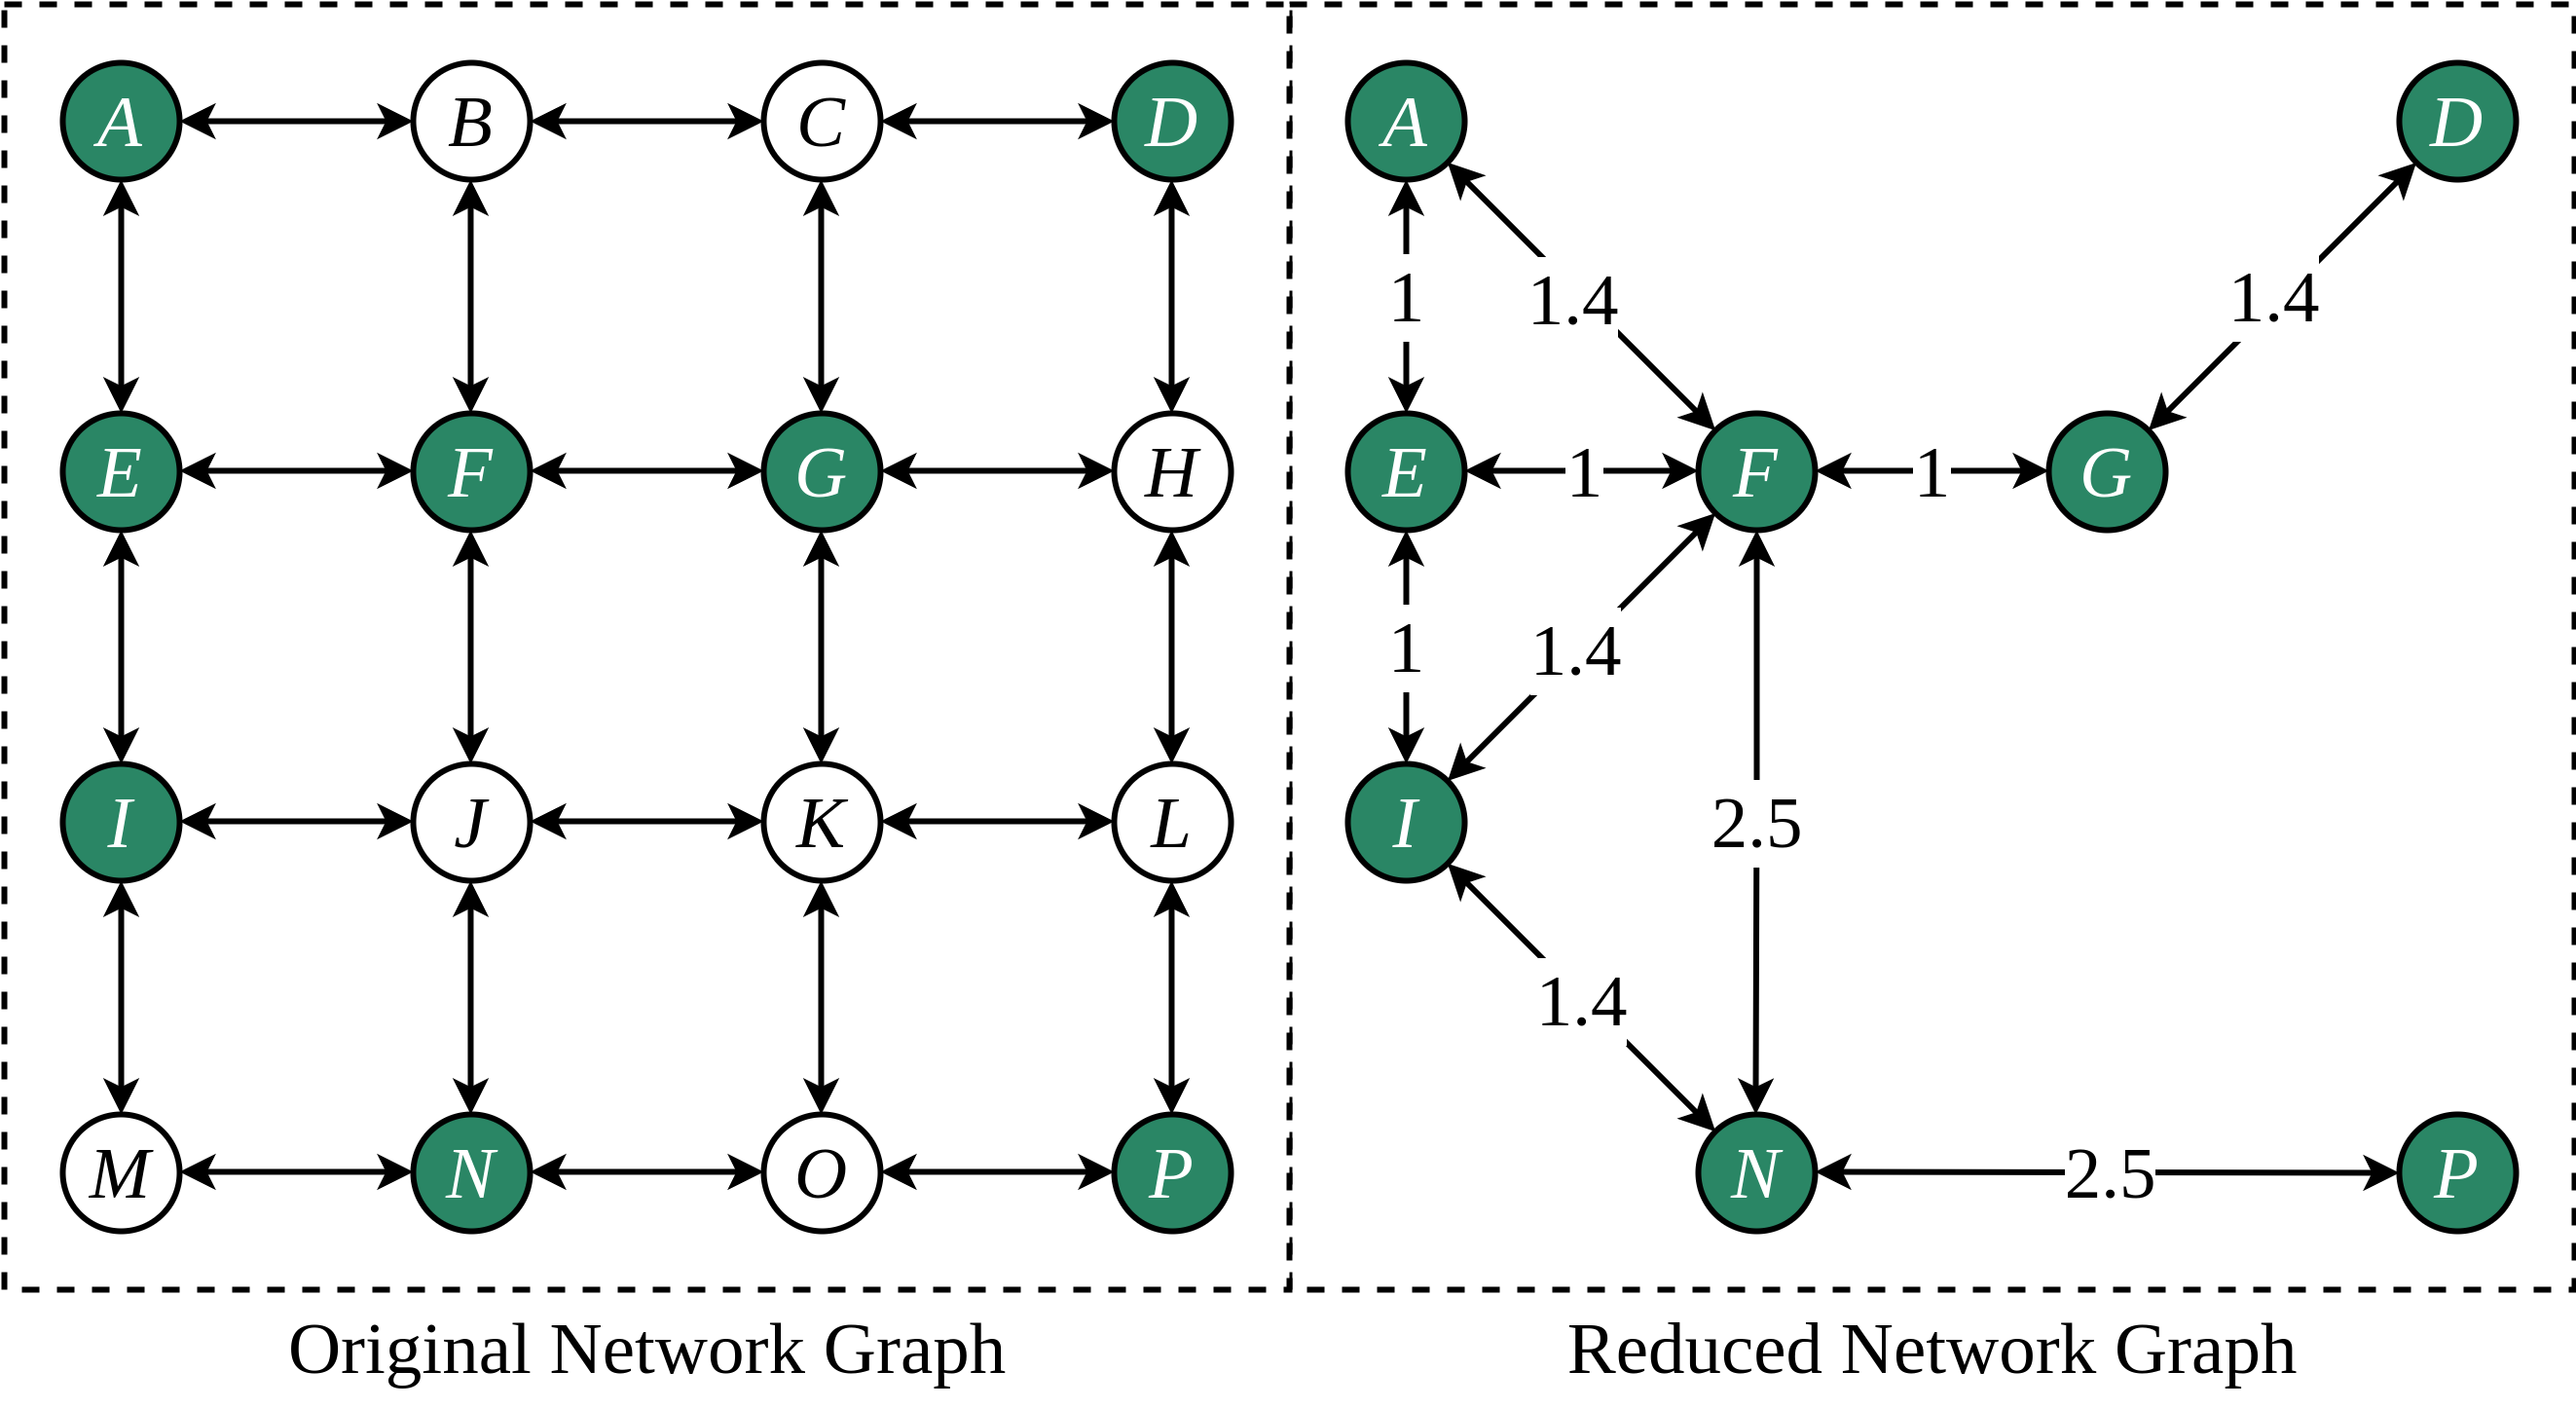
\includegraphics[width = \linewidth]{figs/reduced_sub_network_graph.png}
	\caption{Example original and reduced sub-network graphs. The original graph is a lattice where all edges are valued at 1. The reduced network contains all paths less than or equal to 2.5 between selected nodes as edges.}
	\label{fig:reduced_sub_network_graph}
\end{figure}

\subsection*{Models}

The method requires several models which serve to inform optimal routing. Vehicular, infrastructural, and individual parameters effect the ultimate solution.

\subsubsection*{Vehicles}

Vehicles contribute to routing parameters related to their \glspl{ess} as listed in Table \ref{tab:param_veh}.

\begin{table}[H]
	\centering
	\caption{Vehicle Parameters for Routing}
	\label{tab:param_veh}
	\begin{tabular}{|C{\linewidth*3/8}|C{\linewidth*3/8}|C{\linewidth*2/8}|}
		\hline Parameter & Description & Unit \\
		\hline \gls{ess} Capacity & Accessible energy storage capacity for vehicle & [kWh] \\
		\hline Energy Consumption & Energy required to move the vehicle a given unit of distance & [kJ/km] \\
		\hline Energizing Rate & Rate at which energy can be added to the \gls{ess} at a supply location & [kW] \\
		\hline DC Charge Limits & Lower and upper \gls{soc} bounds for DC charging & [-] \\
		\hline
	\end{tabular}
\end{table}

\subsubsection*{Supply Stations}

Supply infrastructure impacts routing by providing the ability for trips greater than a vehicle's usable range to be completed. Utilizing a supply station resets the vehicle's \gls{soc} to a set level but costs money and time. The cost of the energy supplied is a station level parameter and may vary by location and time. The time added due to energizing is a function of the vehicle and supply equipment maximum energizing rate, the total energy added, and the time spent prior to energizing due to queuing if no equipment is immediately available. The amount of time that a vehicle can expect to queue is a function of the arrival rate of vehicles at a given station, the time taken to energize by those vehicles, the number of supply equipment at the station, and the probability of usability for said equipment. Expected queuing time distributions for different arrival rates and numbers of equipment for DC \gls{ev} chargers are shown in Figure \ref{fig:expected_delay}.

\begin{figure}[H]
	\centering
	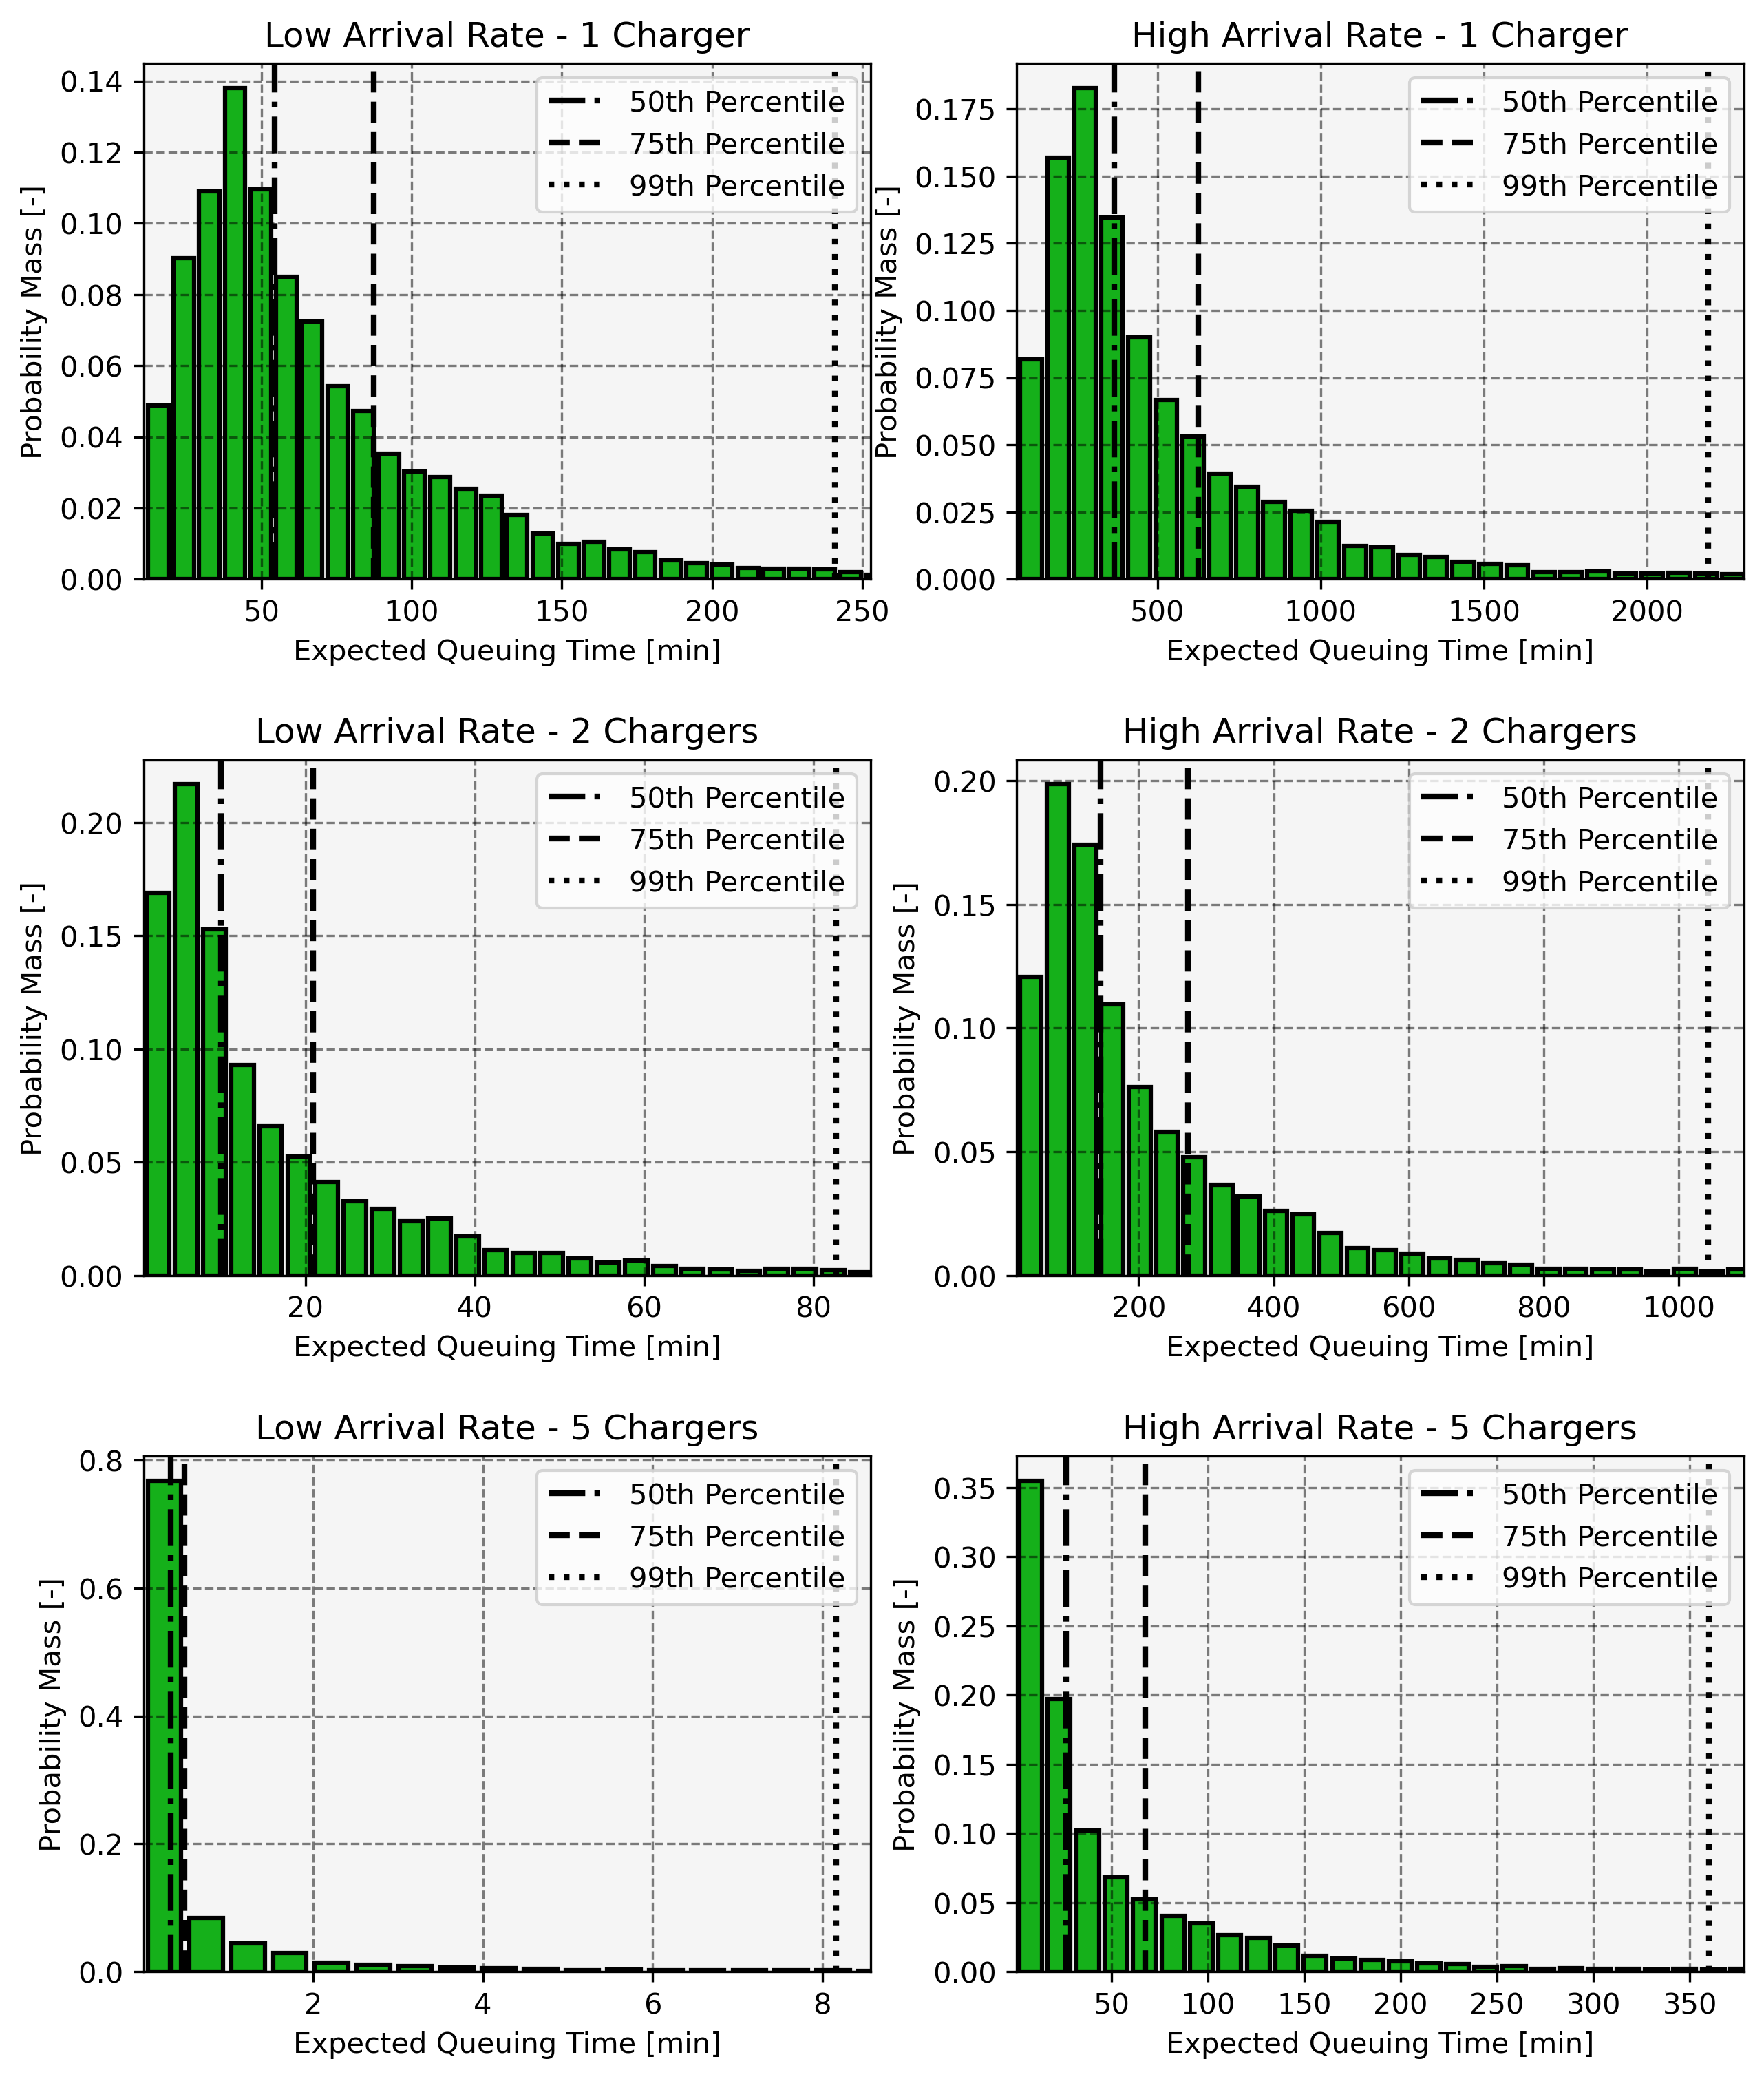
\includegraphics[width = \linewidth]{figs/expected_delay.png}
	\caption{Expected queuing time at charging stations. Low arrival rate is 10 - 60 minutes between arrivals. High arrival rate is 1 - 10 minutes between arrivals. All charge rates are 80 kW and charge events are 60 $\pm$ 15 kWh.}
	\label{fig:expected_delay}
\end{figure}

Expected queuing time is highly determined by variable factors like arrival rate, which must be estimated, and numbers of usable equipment, which is a function of installed equipment and reliability. The amounts of energy purchased are less variable station-to-station for the same powertrain type. The queuing times shown in Figure \ref{fig:expected_delay} were computed using the expected waiting time formula for a M/M/c queue. This approximation is reflective of reality as long trips will begin well before there can be certainty about queues at distant stations. Supply station parameters are listed in Table \ref{tab:param_supply}.

\begin{table}[H]
	\centering
	\caption{Supply Station Parameters for Routing}
	\label{tab:param_supply}
	\begin{tabular}{|C{\linewidth*3/8}|C{\linewidth*3/8}|C{\linewidth*2/8}|}
		\hline Parameter & Description & Unit \\
		\hline Inter-Arrival Time & Time between arrivals at the station & [s] \\
		\hline Service Time & Time taken to supply energy to vehicles & [s] \\
		\hline Servicers & Number of vehicles which can be simultanously serviced & [-] \\
		\hline Usability & Percentage of the time that a given servicer will be usable (accessible and functional) & [-] \\ 
		\hline
	\end{tabular}
\end{table}

\subsubsection*{Drivers}

Given the same physical circumstances, different drivers will evaluate route costs differently. In a basic sense, drivers will weight several factors such as time, money cost, distance, and complexity. Where any important factor is not known precisely drivers will consider a range of outcomes and decide based on an expectation. Driver risk attitude concerns what range of outcomes will be used to compute expected cost. Risk attitude is modeled using a superquantile risk function defined as

\begin{equation}
	S(D, p_0, p_1) = \frac{1}{p_1 - p_0}\int_{p_0}^{p_1}Q(D, \alpha)\ d\alpha \label{eq:superquantile}
\end{equation}

where $D$ is a distribution, $p_0$ and $p_1$ are the boundaries of the range of probabilities considered in the expectation, and $Q$ is the quantile function of $D$. The superquantile is, thus, the mean value of a distributed quantity within a range of probability. Drivers with an aggressive risk attitude will consider a low range of probabilities, drivers with a neutral attitude will consider a central range, and drivers with a cautious attitude will consider a high range. Thus, a driver's perceived route cost is computed via taking the superquantile of a weighted sum of route costs. Driver parameters are listed in Table \ref{tab:param_driver}.

\begin{table}[H]
	\centering
	\caption{Supply Station Parameters for Routing}
	\label{tab:param_driver}
	\begin{tabular}{|C{\linewidth*3/8}|C{\linewidth*3/8}|C{\linewidth*2/8}|}
		\hline Parameter & Description & Unit \\
		\hline Route Cost Weights $W$ & Set of multipliers for route costs to be used in computation of weighted sum & [-] \\
		\hline Probability Range $(p_0, p_1)$ & Range of probabilities for superquantile function & [-] \\
		\hline
	\end{tabular}
\end{table}

\subsection*{Routing}

The purpose of optimal routing is to find the "shortest-paths" from a given origin $o \in V$ to a set of destinations $D \in V$ on a graph $G = \{V, E\}$. The output of the routing algorithm is tree $P$ containing the shortest feasible paths from the origin to all destinations as edges. The objective of routing between $i$ and $j$ is

\begin{equation}
	\min_{U \in \overline({U}_{i,j})}\ \mathbb{E}[J(S_0, U)]
\end{equation}

where

\begin{equation}
	J(U) = \sum_{k = 0}^M w_k\phi_k(s_{0,k}, U)
\end{equation}

s.t.

\begin{equation}	
	b^w_l \leq \mathbb{E}\left[\int_0^t \Phi_w(S_0, U)dt\right] \leq b^w_u\quad \forall t \in T
\end{equation}

where $S_0$ is the vector of route states, $U$ is a control (route) between $i$ and $j$, $\overline{U}_{i,j}$ is the set of possible routes between $i$, and $j$, $\Phi_w$ is the cost function for route weight $w \in W$, and $\mathbb{E}$ denotes an expectation and is computed as in \eqref{eq:superquantile}. The optimal routes may be found using a stochastic implementation of the Dijkstra or Bellman-Ford algorithms. In either case route states $S$ are initialized and stored as vectors containing $N$ discreet variables. An empirical distribution $D$ for a state vector can be computed from a histogram of the values. States can be changed at nodes and edges. Routes are considered feasible if the expectations of all states remain within set bounds. Comparison between routes is performed using expectation of cost.

\subsection*{Accessibility Metric}

In the presented framework accessibility can be computed in general for a region or in specific for a given origin within the region. In either case, the regional \gls{rsng}, travel mode, mode-specific infrastructure, and traveler must be modeled. For region $R$ with a set of $N$ selected nodes $O = \{O_1, O_2, \dots, O_N\}$ and corresponding set of importance weights $W = \{W_0, W_1, \dots, W_N\}$ and optimal path trees $P = \{P_1, P_2, \dots, P_N\}$, accessibility metric $A$ is the weighted mean

\begin{equation}
	A(R) = \frac{1}{N^2}\sum_{i = 0}^{N} \sum_{j = 0 }^{N} W_iW_jP_{i,j} \label{eq:a}
\end{equation}

where $P_{i,j}$ is the cost of the optimal path from $O_i$ to $O_j$. The specific accessibility metric $A(R, o)$ can be computed for region $R$ and origin $o$ by setting $W = \{W_o\}$ and $P = \{P_o\}$. Thus, a direct comparison in accessibility between regions, origins, travel modes, travelers, infrastructure deployments, or any of those mentioned in combination can be conducted.

The accessibility metric $A$ is of the proximity type concerned, primarily, with the expected cost to transit edges between pre-determined O/D pairs. In contrast with accessibility studies focused on routine travel behavior, this study is focused on non-routine long trips. It is assumed that travelers, when considering non-routine long trips have a specific destination in mind and would not consider roughly equidistant cities as fungible destinations. Rather, it is assumed that, having determined to travel to a given location, the traveler will then decide on mode with roughly equivalent cost modes being fungible.

A transportation accessibility metric should have land-use, transportation, temporal, and individual components \cite{Karst_2003}. Metric $A$ contains all listed components. The land-use within a region has two principle effects on $A$. First, for a multi-city region, specific accessibility should vary within the region with peripheral cities experiencing worse regional access than central cities. Second, geographically large and/or sparse regions should experience worse accessibility than compact regions. The transportation infrastructure determines the efficacy of various modes. Where only vehicular travel is concerned, the mode choice is reduced to vehicle choice. Vehicle mode-specific infrastructure is not necessarily the same for all vehicles of a given fuel type but is necessarily different between fuel types thus making mode determinative even if all modes are vehicular. The temporal component of $A$ arises from the schedules of public transportation services and road traffic patterns. Finally the individual component is the traveler risk attitude as in \eqref{eq:superquantile}.

\section*{California Case Study}

\subsection*{Background}

The state of California contains large population centers distributed across the state with major road transportation corridors forming connections between them and with population centers in adjacent states. This case study concerns the accessibility of California for non-routine long road trips. For the purposes of analysis, 15 important cities in California and adjacent states were selected. For the purposes of scope limitation, the non-California locations are represented by the most-likely departure locations at the California state line. These locations are enumerated in Table \ref{tab:locations}.

\begin{table}[H]
	\centering
	\caption{Locations Considered for Long Trip Accessibility}
	\label{tab:locations}
	\begin{tabular}{|C{\linewidth * 1 / 3}|C{\linewidth * 2 / 3}|}
		\hline Index & Location \\
		\hline 0 & Crescent City \\
		\hline 1 & Yreka \\
		\hline 2 & Redding \\
		\hline 3 & Chico \\
		\hline 4 & Reno (State Line) \\
		\hline 5 & Sacramento \\
		\hline 6 & Stockton \\
		\hline 7 & San Francisco \\
		\hline 8 & San Jose \\
		\hline 9 & Fresno \\
		\hline 10 & Las Vegas (State Line) \\
		\hline 11 & Bakersfield \\
		\hline 12 & Los Angeles \\
		\hline 13 & Phoenix (State Line) \\
		\hline 14 & San Diego \\
		\hline
	\end{tabular}
\end{table}

These locations were chosen either because they are, themselves, important destinations in California or because they are the closest points in California to important destinations in neighboring states. For long trips, \glspl{bev} will rely on DC charging stations. The locations of all DC charging stations in California were scraped from AFDC \cite{afdc_2023} and include proprietary stations such as Tesla Superchargers and the Rivian Adventure network as well as non-proprietary stations such as those operated by ChargePoint, Electrify America, eVgo, and others. The selected locations and DC charging stations are mapped in Figure \ref{fig:california_atlas}.

\begin{figure}[H]
	\centering
	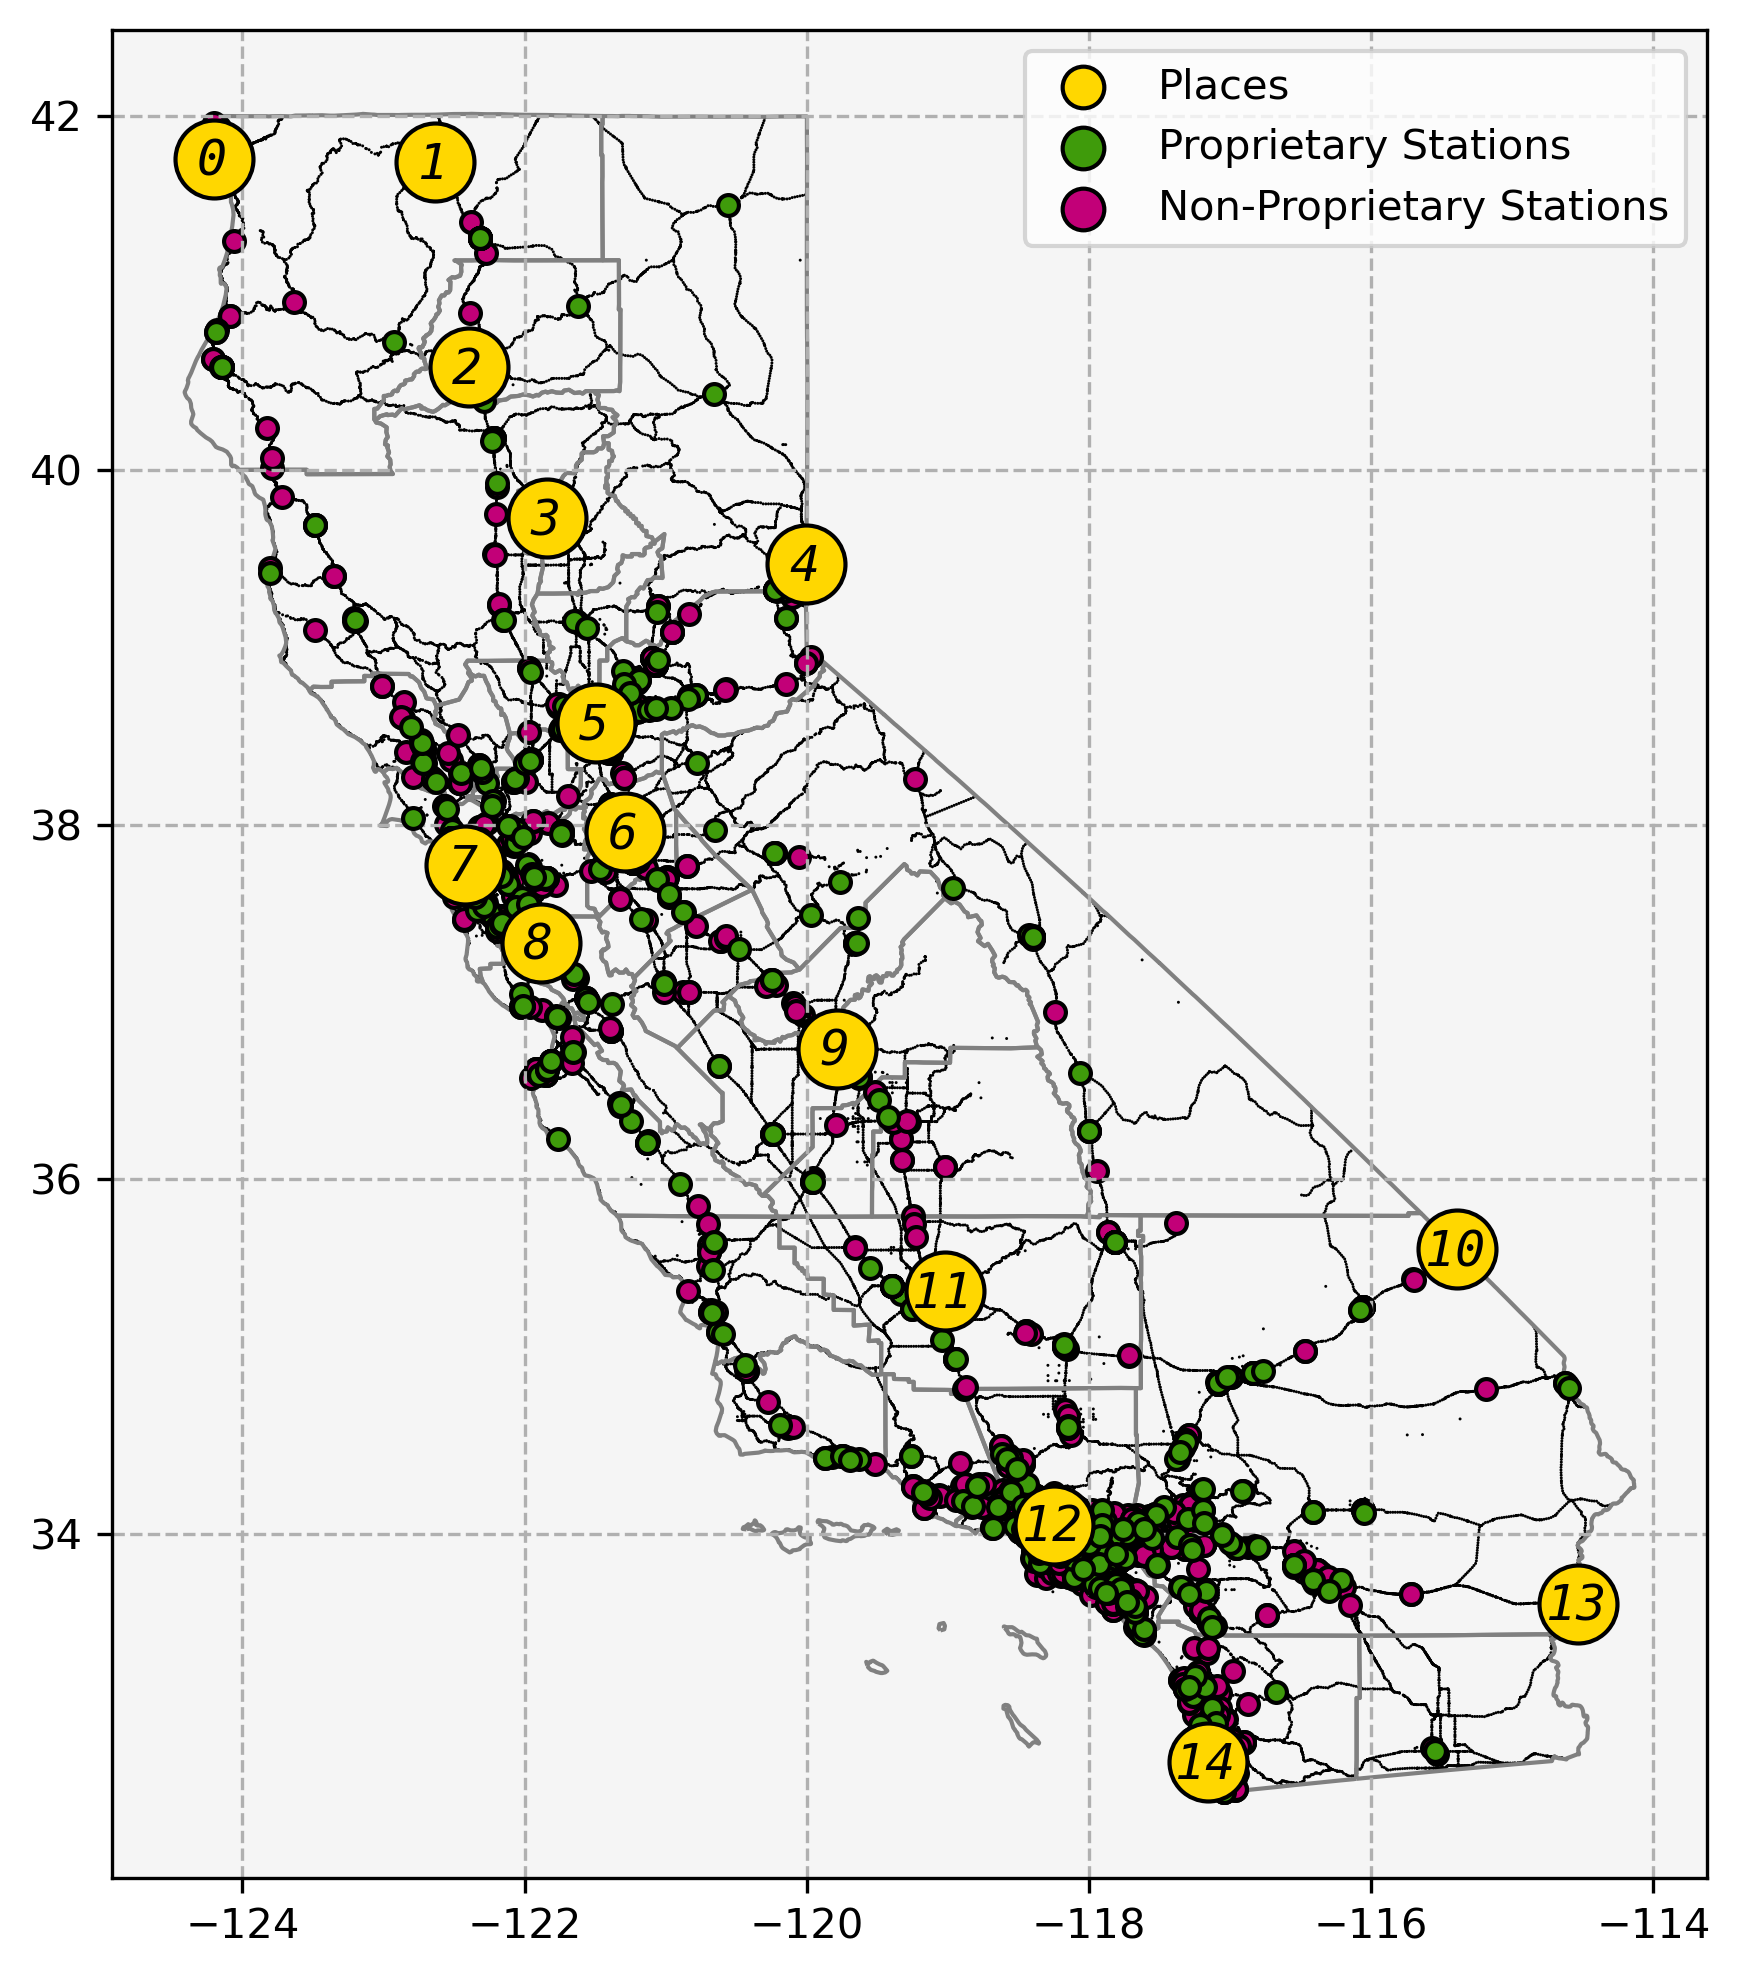
\includegraphics[width = \linewidth]{figs/California_Places_Chargers.png}
	\caption{Selected locations and charging stations for California case study}
	\label{fig:california_atlas}
\end{figure}

The proprietary and non-proprietary networks in California are not equivalent and should not be treated as such. There are 403 Tesla and 78 Rivian DC charging stations in the state as compared to 1,425 non-proprietary DC charging stations. The non-Tesla overwhelmingly use combination CCS/ChaDeMo plugs as defined by SAE J1772 \cite{SAE_J1772} which reflect the ports on the overwhelming number of non-Tesla \glspl{bev}. By contrast, Tesla chargers and vehicles use the NACS standard as defined by SAE J3400 \cite{SAE_J3400}. The Tesla and non-Tesla systems are increasingly interoperable with the aid of adapters and may become natively so as standard in the future but should be considered separately in the present. Tesla drivers use Tesla DC chargers almost exclusively \cite{Visaria_2022} and CCS/ChaDeMo to NACS adapters are more common than their counterparts. The Rivian Adventure network is technically interoperable with other J1772 vehicles but is set aside for the exclusive use of Rivian vehicles. The purpose of the Rivian Adventure network is to allow for Rivian vehicles to charge in remote locations and is not intended to be the only network used by them.

The difference between the Tesla DC charging network and the non-proprietary network extends from function to form. Built out as an investment to entice sales of Tesla vehicles and, until recently, exclusive to them, the Tesla network is technically superior with higher rate and more reliable chargers \cite{Rempel_2023, Kozumplik_2022}. Non-proprietary networks have, so far, been subsidy driven \cite{Gamage_2023} and have responded to incentives to form a widely distributed but thin presence. A stark contrast is seen when examining the ratio of chargers to stations. In California there are 403 Tesla DC charging stations with a total of 6,277 DC chargers for an average of 15.6 chargers per station. Among non-proprietary networks there are a total of 1,425 stations with 3,667 chargers for an average of 2.6 per station. The distributions of chargers per station for Tesla and non-proprietary networks are shown in Figure \ref{fig:network_histograms}.

\begin{figure}[H]
	\centering
	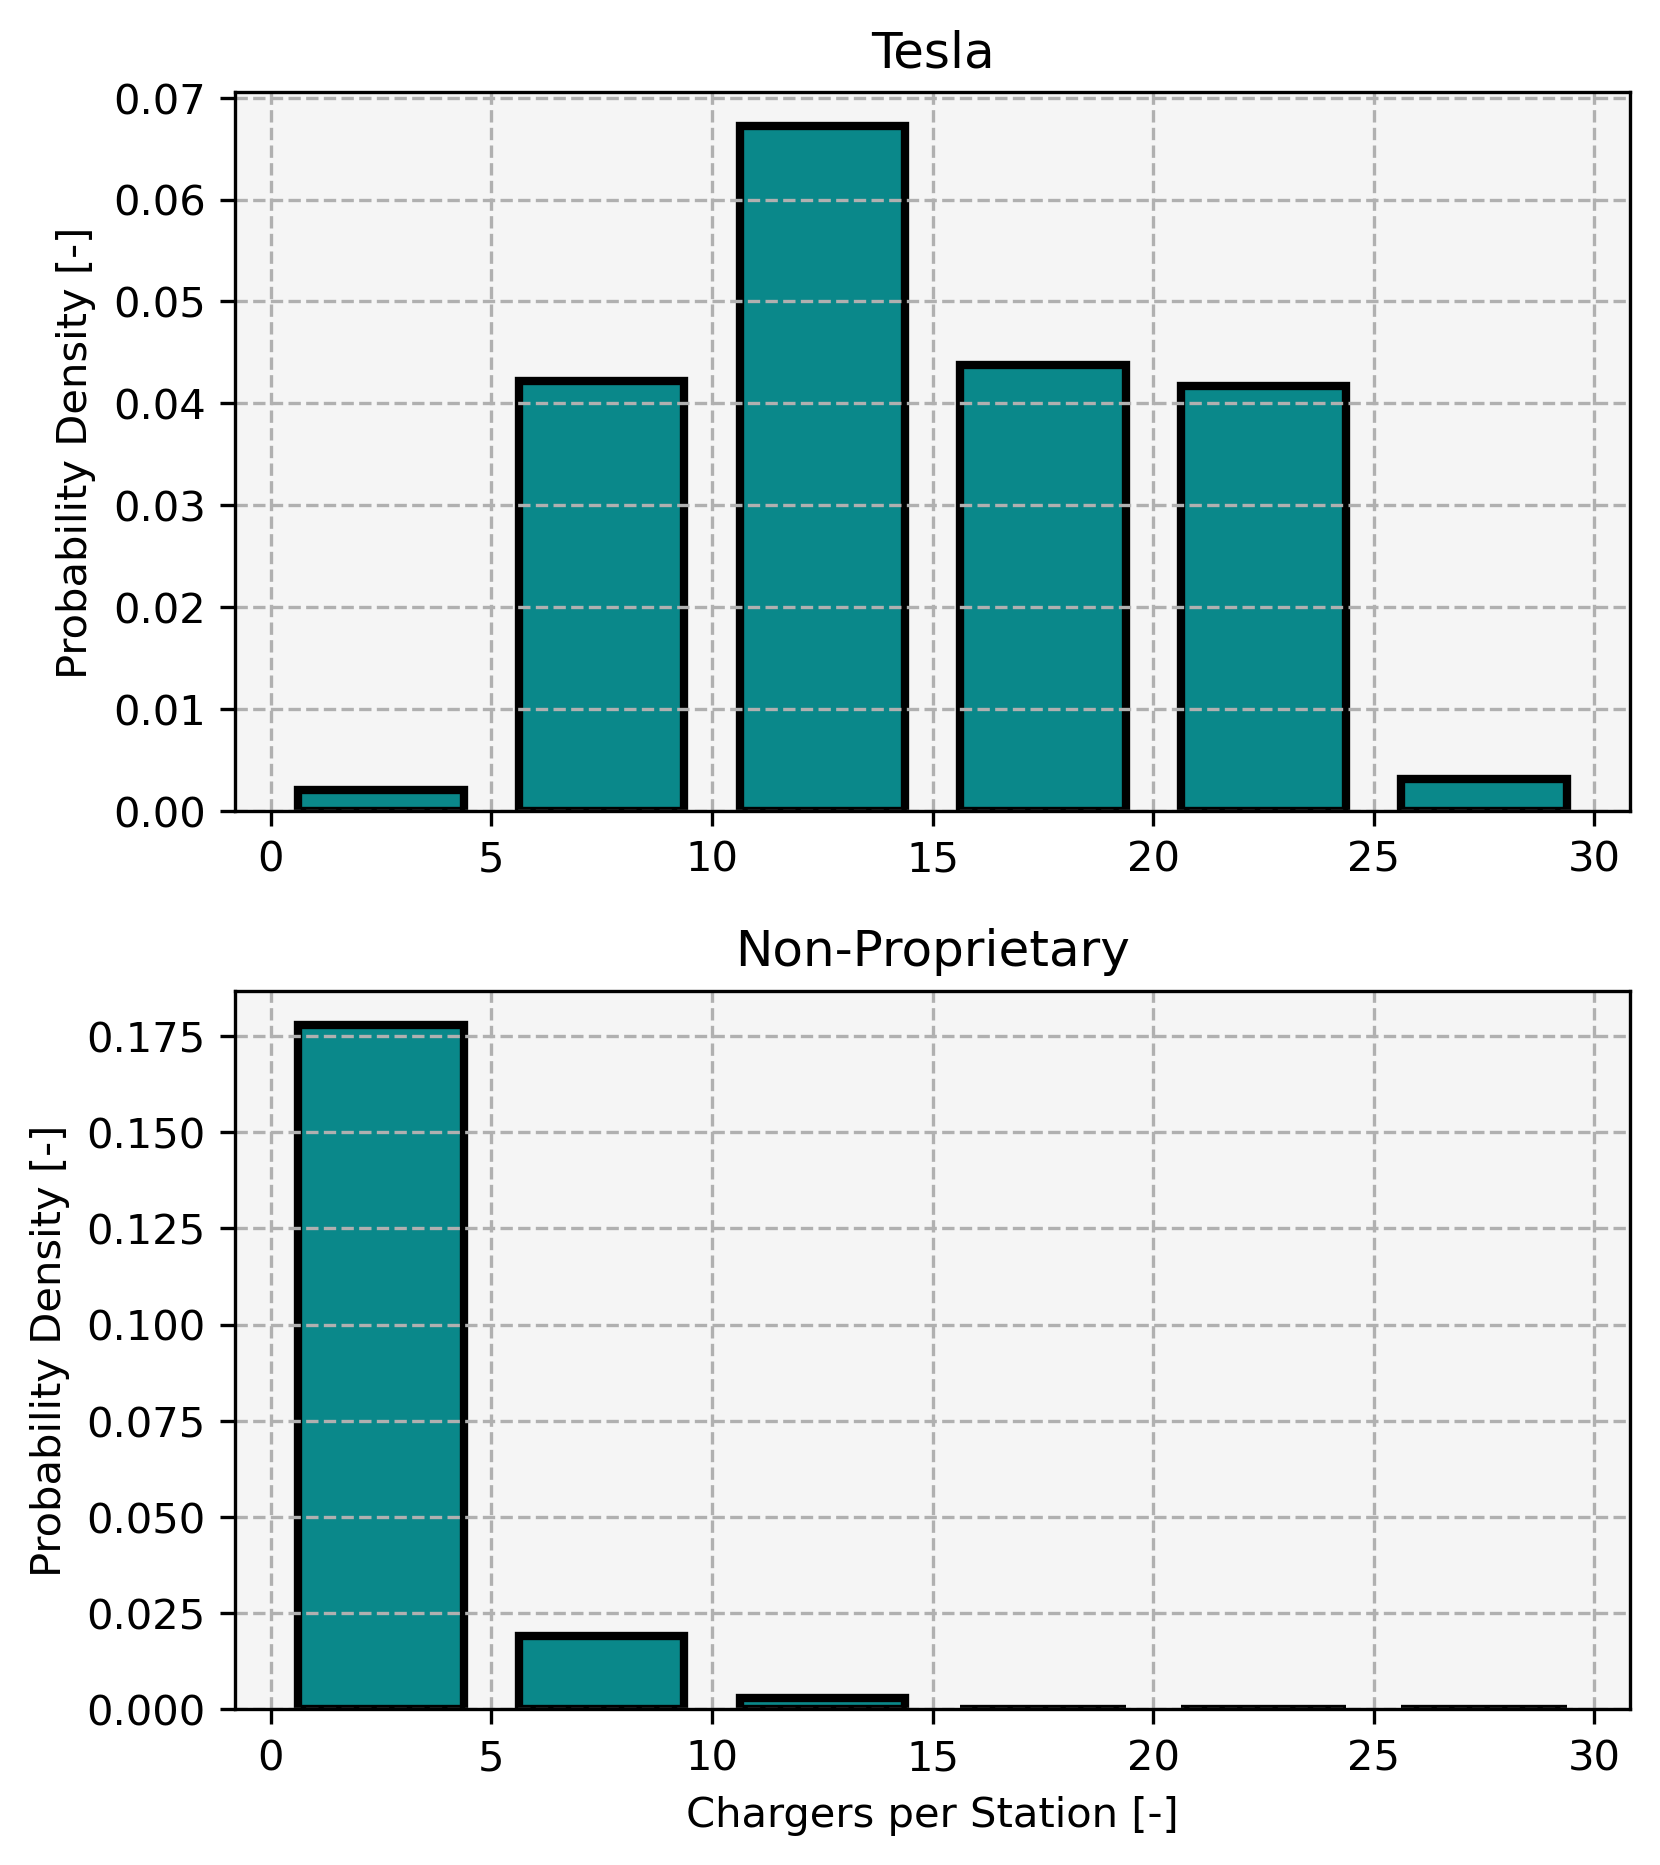
\includegraphics[width = \linewidth]{figs/California_Charger_Network_Histograms.png}
	\caption{Distributions of chargers per station for Tesla and non-proprietary networks in California.}
	\label{fig:network_histograms}
\end{figure}

As demonstrated in Figure \ref{fig:expected_delay}, the number of chargers at a station has a major effect on expected delay time as well as determining the importance of individual equipment failure. It should also be mentioned that \glspl{icev} utilize a third and completely separate network of supply stations. There are estimated to be over 8,000 gasoline stations in California \cite{CEC_2022} and these are widely and proportionally distributed. Because no public database for the locations of gasoline stations in the state exists, and due to their ubiquity it is assumed in this study that \gls{icev} driver optimal paths will not be effected by fueling station availability and that such stations will be available wherever needed. For this reason, \glspl{icev} are assumed to take the "direct" path between cities where \glspl{bev} need to find optimal paths on the California \gls{rsng}.

\subsection*{Example}

Consider, as an example, the following four scenarios for a driver based out of Fresno:


\begin{compactenum}
	\item Risk neutral driver using a generic \gls{icev}.
	\item Risk neutral driver using a Tesla Model 3 with an 80 kWh battery capable of charging at a max rate of 170 kW. The driver uses the Tesla DC station network exclusively and this network has high charger up-time (97\%). Vehicles are expected to arrive at stations on the order of once every 10 to 30 minutes.
	\item Risk-cautious driver using a Chevrolet Bolt EV with an 65 kWh battery capable of charging at a max rate of 55 kW. The driver uses various non-proprietary networks and these networks have low charger up-time (75\%). Vehicles are expected to arrive at stations on the order of once every 10 to 60 minutes.
	\item Risk-aggressive driver using a Chevrolet Bolt EV with an 65 kWh battery capable of charging at a max rate of 55 kW. The driver uses various non-proprietary networks and these networks have low charger up-time (75\%). Vehicles are expected to arrive at stations on the order of once every 10 to 60 minutes.
\end{compactenum}

Each of these drivers will have a different experience of California's road transportation system for long trips. The neutral-expectations of time to reach each of the selected locations are provided in Table \ref{tab:scenarios} (driver is required to arrive at each destination with  at least 50\% \gls{soc}).


\begin{table}[H]
	\centering
	\caption{Neutral expectation of hours to locations from Fresno for example scenarios.}
	\label{tab:scenarios}
	\begin{tabular}{|C{.17\linewidth}|C{\linewidth * 1 / 5}|C{\linewidth * 1 / 5}|C{\linewidth * 1 / 5}|C{.23\linewidth}|}
		\hline Index & \gls{icev} & Model 3 Neutral & Bolt Cautious & Bolt Aggressive \\
		\hline 0 & 9.02 & 9.89 & NaN & 15.27 \\
		\hline 1 & 7.16 & 7.47 & NaN & 10.24 \\
		\hline 2 & 5.71 & 6.14 & NaN & 9.09 \\
		\hline 3 & 4.46 & 4.69 & 9.63 & 6.72 \\
		\hline 4 & 4.67 & 5.00 & 8.83 & 7.03 \\
		\hline 5 & 2.82 & 2.82 & 4.52 & 4.42 \\
		\hline 6 & 2.09 & 2.09 & 2.09 & 2.09 \\
		\hline 7 & 3.32 & 3.29 & 5.05 & 4.71 \\
		\hline 8 & 2.71 & 2.71 & 4.86 & 4.54 \\
		\hline 9 & 0.00 & 0.00 & 0.00 & 0.00 \\
		\hline 10 & 5.86 & 6.29 & NaN & 9.93 \\
		\hline 11 & 1.64 & 1.64 & 1.64 & 1.64 \\
		\hline 12 & 3.32 & 3.65 & 5.78 & 5.71 \\
		\hline 13 & 6.81 & 7.52 & 14.69 & 11.52 \\
		\hline 14 & 5.28 & 5.72 & 10.26 & 8.74 \\
		\hline
	\end{tabular}
\end{table}

The example drivers have very different experiences and perceived experiences. While the \gls{icev} driver can take the "direct" path (not deviating to find a station), the \gls{bev} drivers have to deviate from the "direct" path and require substantial time to charge. However, there is quite significant disparity within the set of proposed \gls{bev} drivers. For destinations which are within full-charge range, there is no difference. However, due to the lower range, lower max charge rate, and lower infrastructure reliability for the Bolt, the differentials between it and the Model 3 can be tremendous, especially for remote locations. For 4 remote locations (Crescent City, Yreka, Redding, and Las Vegas (State Line)) the cautious Bolt driver would consider an out-of-charge event sufficiently probable to make the journey not feasible, while the aggressive Bold driver would consider the journey arduous. It is worth noting, also, that the \gls{icev} and Model 3 are able to take more direct routes although the differences are not as pronounced. Table \ref{tab:scenarios_nc} shows the optimal route times with charging/fueling times removed.

\begin{table}[H]
	\centering
	\caption{Neutral expectation of hours to locations from Fresno for example scenarios without charging/fueling time.}
	\label{tab:scenarios_nc}
	\begin{tabular}{|C{.17\linewidth}|C{\linewidth * 1 / 5}|C{\linewidth * 1 / 5}|C{\linewidth * 1 / 5}|C{.23\linewidth}|}
		\hline Index & \gls{icev} & Model 3 Neutral & Bolt Cautious & Bolt Aggressive \\
		\hline 0 & 8.61 & 8.76 & NaN & 9.03 \\
		\hline 1 & 6.63 & 6.79 & NaN & 6.79 \\
		\hline 2 & 5.14 & 5.74 & NaN & 5.33 \\
		\hline 3 & 4.31 & 4.39 & 5.03 & 4.49 \\
		\hline 4 & 4.59 & 4.67 & 4.66 & 4.80 \\
		\hline 5 & 2.71 & 2.82 & 2.81 & 2.82 \\
		\hline 6 & 2.00 & 2.09 & 2.09 & 2.09 \\
		\hline 7 & 2.96 & 3.07 & 3.21 & 3.11 \\
		\hline 8 & 2.53 & 2.71 & 3.15 & 2.94 \\
		\hline 9 & 0.00 & 0.00 & 0.00 & 0.00 \\
		\hline 10 & 5.82 & 5.87 & NaN & 5.91 \\
		\hline 11 & 1.61 & 1.64 & 1.64 & 1.64 \\
		\hline 12 & 3.26 & 3.32 & 3.32 & 3.32 \\
		\hline 13 & 6.67 & 6.81 & 7.16 & 7.01 \\
		\hline 14 & 5.25 & 5.28 & 5.28 & 5.36 \\
		\hline
	\end{tabular}
\end{table}

The differences in expected travel time between the \gls{icev} and Model 3 are relatively small and in the range of 5-10\% of travel time, a testament to Tesla's DC station network. Some would argue that this difference is unimportant as Tesla drivers can charge their vehicles while stopping for meals or during other natural breaks. This logic has been used to show that \glspl{bev} may approach convenience parity with \glspl{icev} in good circumstances \cite{Dixon_2020}. However, where such breaks are optional for \gls{icev} drivers, they are mandatory for \gls{bev} drivers and must be taken at specific points throughout the trip to coincide with charging. The loss of optionality must be accounted an inconvenience even if breaks would be taken in any event.

\subsection*{Experiment}

In order to gain a broader understanding of the effects of vehicular, infrastructural, and individual characteristics on transportation accessibility for long trips in California a designed experiment was conducted on the parameters in Table \ref{tab:exp_parameters}.

\begin{table}[H]
	\centering
	\caption{Parameters and levels for designed experiment}
	\label{tab:exp_parameters}
	\begin{tabular}{|C{.5\linewidth}|C{.5\linewidth}|}
		\hline Parameter & Levels \\
		\hline Charger Network & [Tesla, Non-Proprietary] \\
		\hline Range/Max Charge Multiplier & [1, 1.25, 1.5] \\
		\hline Charger Reliability & [.75, .85, .95] \\
		\hline Risk Attitude & [Cautious, Neutral, Aggressive] \\
		\hline
	\end{tabular}
\end{table}

The rationale behind the selection of levels is as follows. As mentioned previously, the Tesla and non-proprietary DC charging networks are, presently, effectively separate and unequal entities. The base vehicle models in this study are the Chevrolet Bolt and Tesla Model 3 both of which are low-end vehicles for their category with more expensive models coming with higher battery capacities and charge rates \cite{AFDC_EVs_2023}. The range of reliability rates was taken from references \cite{Rempel_2023} with an aspirational high reliability rate added. Finally, risk attitudes were modeled on the theoretical basis outlined in the Methods section using \eqref{eq:superquantile} with Cautious ($p_0 = .5,\ p_1 = 1$), Neutral ($p_0 = 0,\ p_1 = 1$), and Aggressive ($p_0 = 0,\ p_1 = .5$) drivers.

The metric used for comparison is accessibility as in \eqref{eq:a} relative to an \gls{icev}. In each case the optimal-path tree $P$ is computed using the constrained implementation of Dijkstra's method as described in the Methods section with sample vectors of length 30.

\newpage

\printbibliography

\end{multicols}

\end{document}

%\subsection*{Random Graph Example}
%
%The optimal routing method in this study accounts for factors which influence road vehicle accessibility and derive from vehicular, infrastructural, and behavioral parameters. Important vehicular parameter for accessibility is range which determines which locations can be reached with and without charging. Important infrastructural parameters such as the number and locations of charging stations, usability rates, and expected delay times. Important behavioral parameters include risk attitude parameters as in \eqref{eq:superquantile}. These factors influence routing individually and via interactions as demonstrated on a randomly generated graph.
%
%A random graph of 100 nodes, 15 containing charging stations within a 100 km by 100 km square was generated with a random node selected as the origin. Edge probabilities were defined relative to a characteristic distance using
%
%\begin{equation}
%	P(e) = \exp(-L(e)/d)
%\end{equation}
%
%where $e$ is an edge, $L(e)$ is the distance of edge $e$, and $d$ is a characteristic distance set to 200 km for this example. In this example the vehicle has a range of 460 km and each charging station has one charger and a low vehicle arrival rate. Figure \ref{fig:interactions} show how $R$ is effected by different usability rates and risk attitudes.
%
%\end{multicols}
%
%\begin{figure}[H]
%	\centering
%	\begin{subfigure}{.4\linewidth}
	%		\centering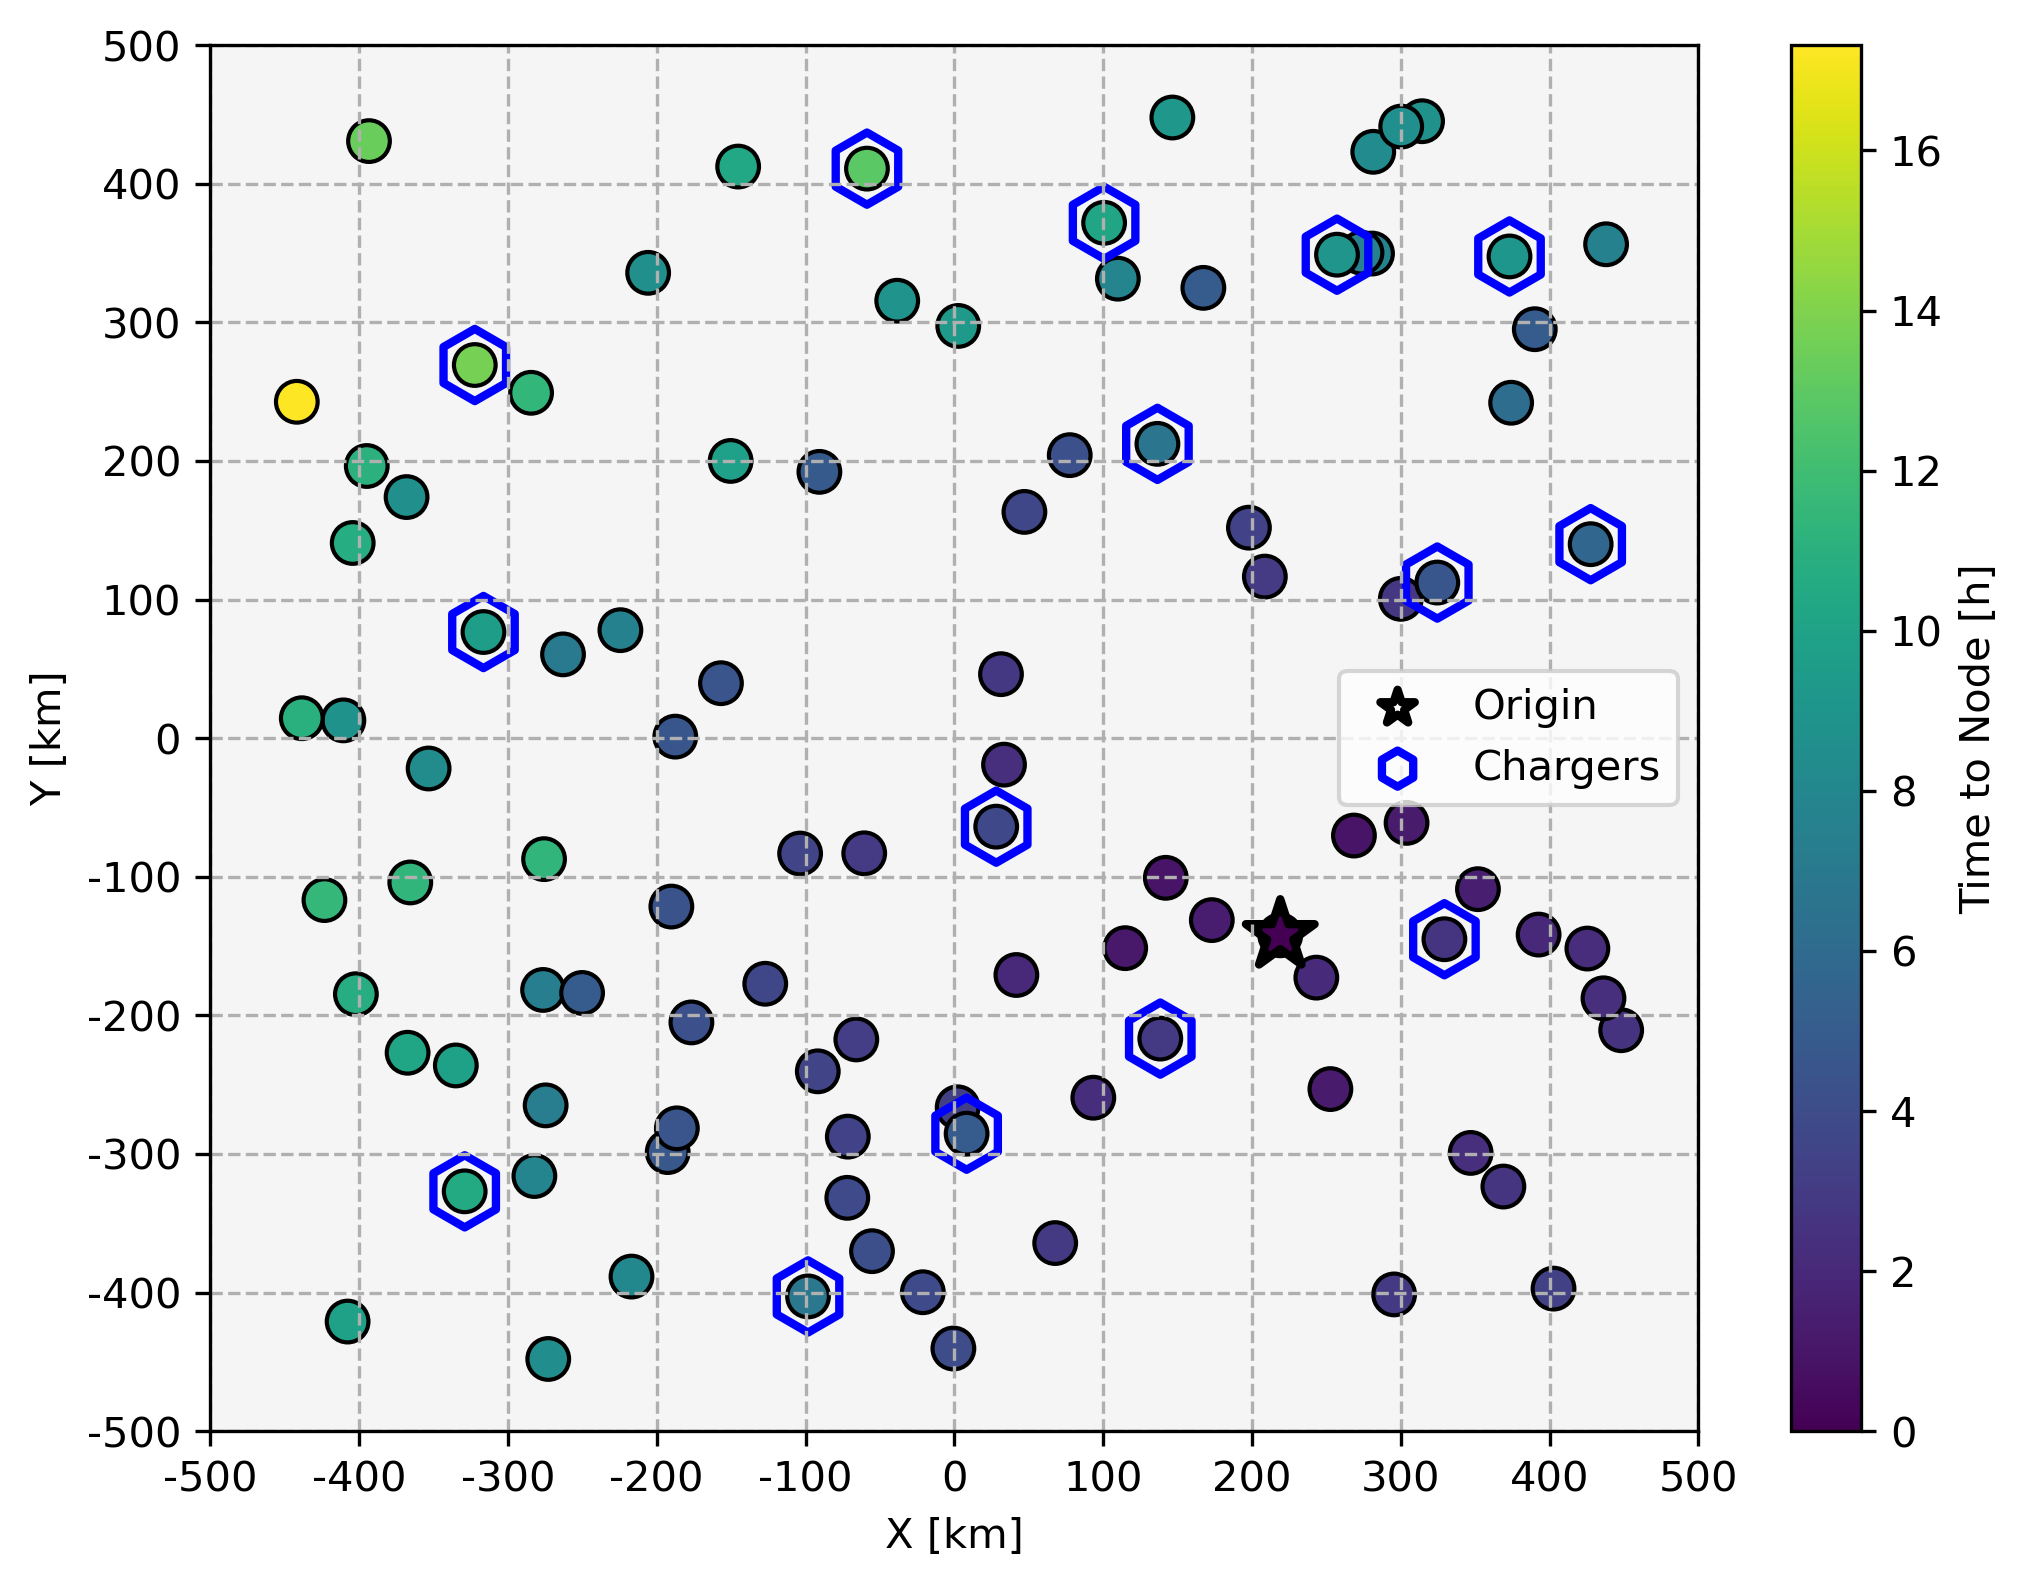
\includegraphics[width = \linewidth]{figs/interactions_ha.png}
	%		\captionsetup{width=.8\linewidth}
	%		\caption{High charger usability and aggressive risk attitude}
	%	\end{subfigure}%
%	\begin{subfigure}{.4\linewidth}
	%		\centering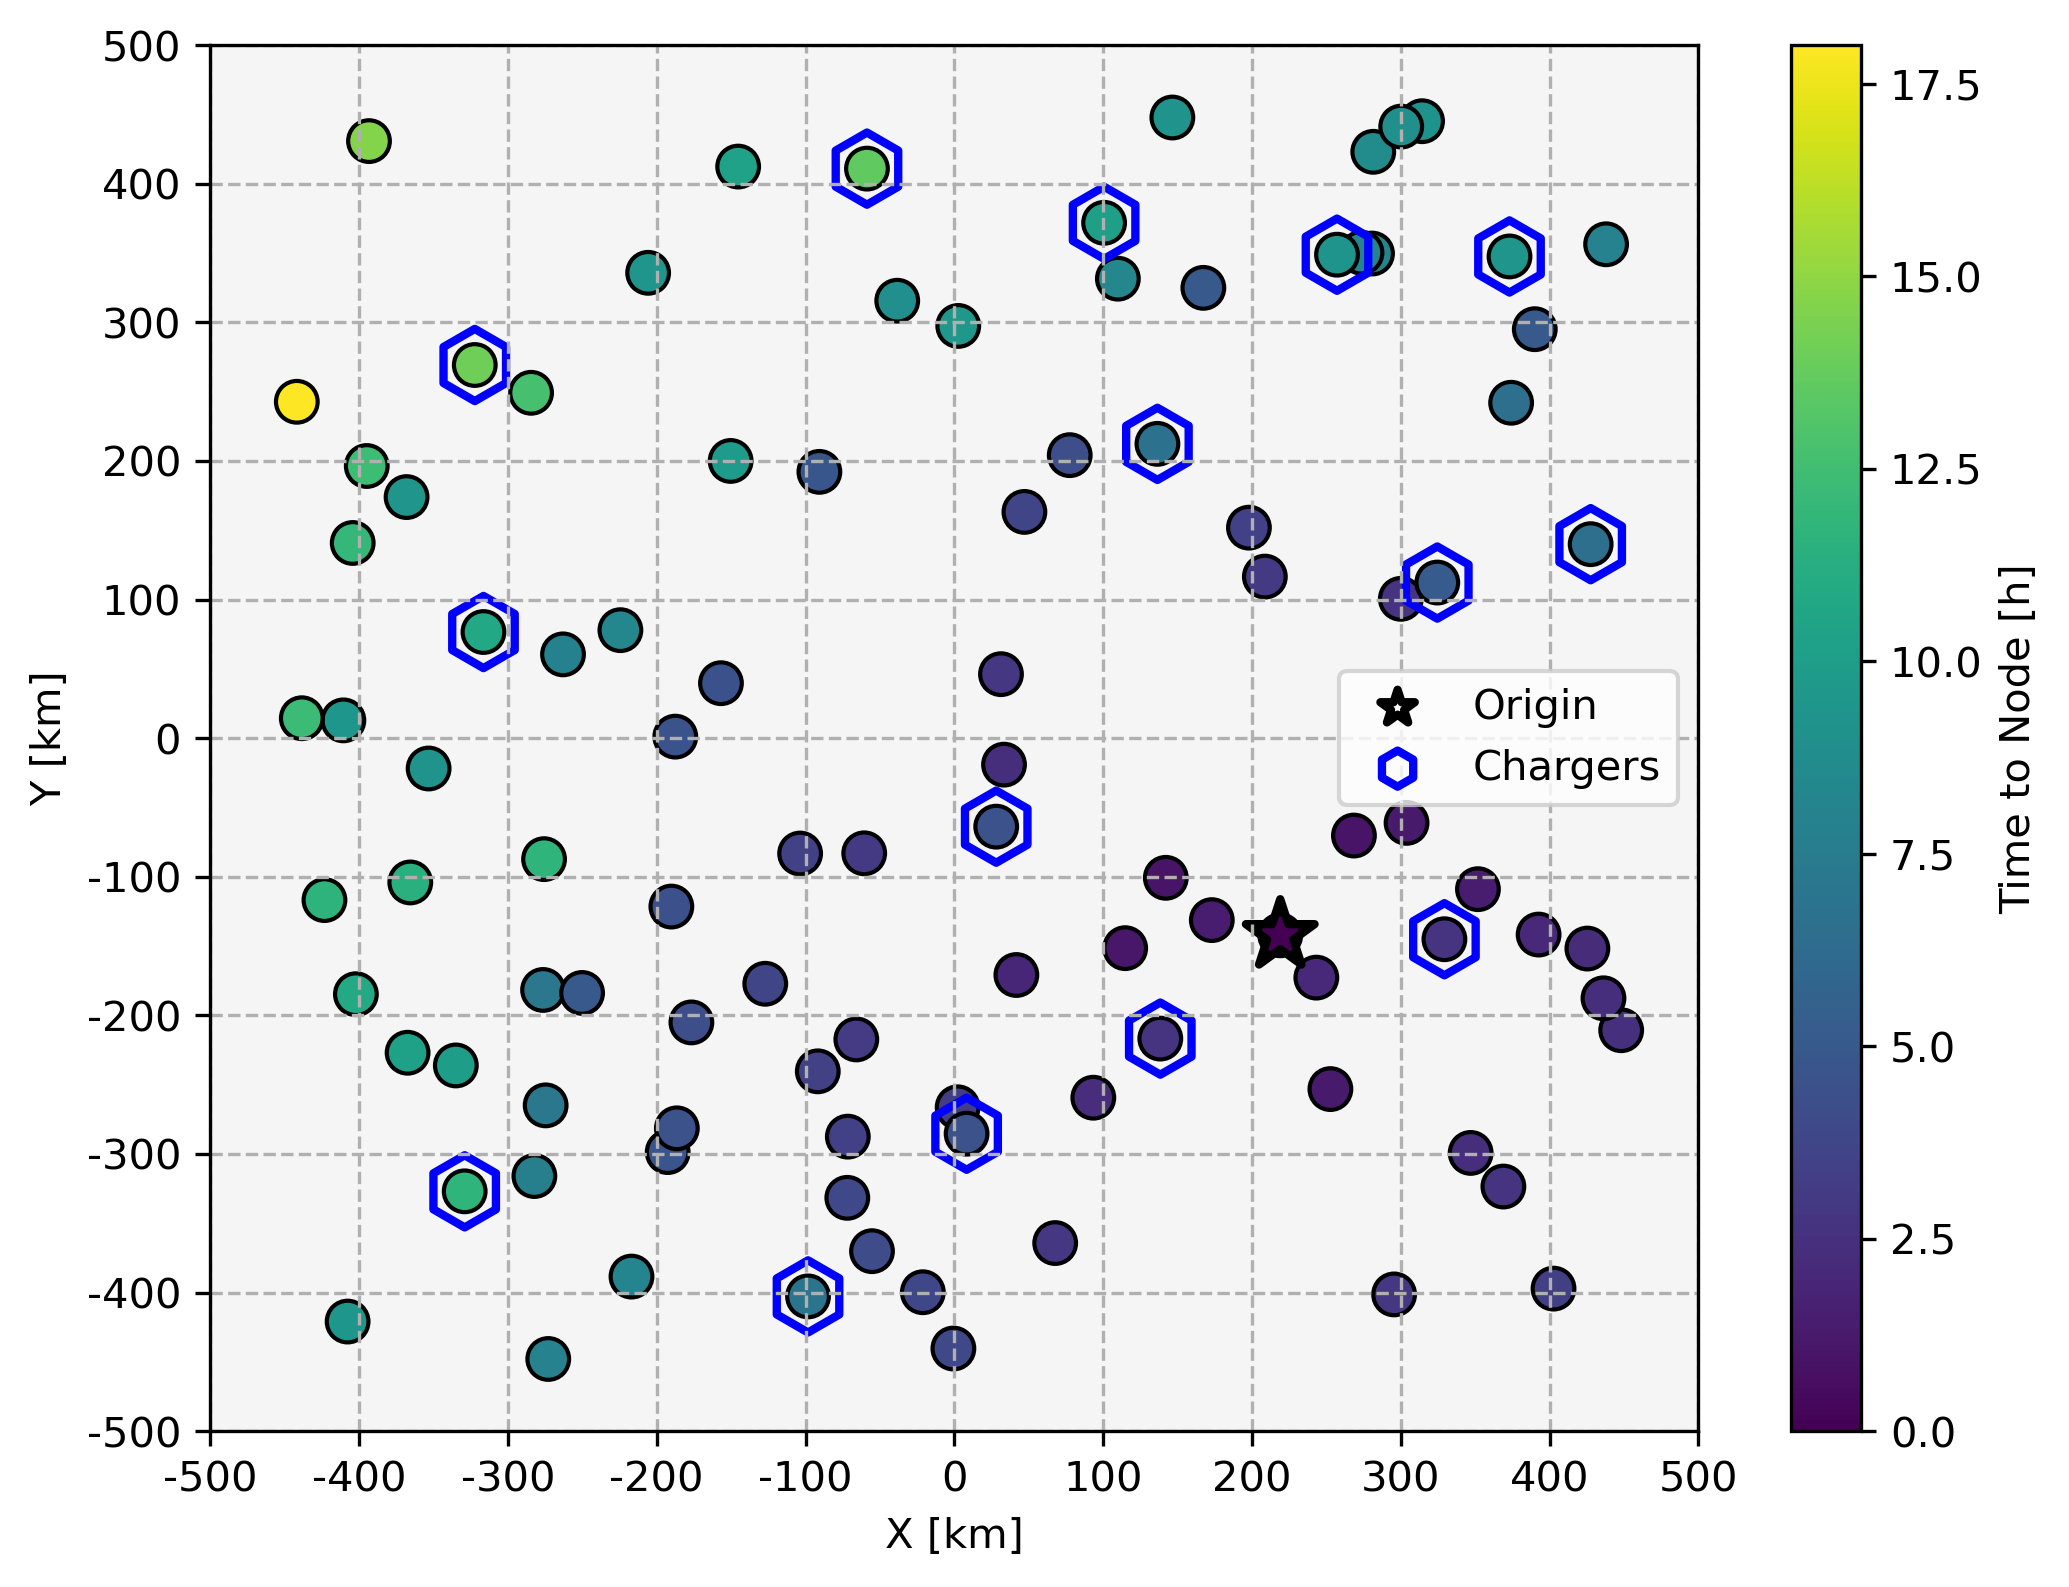
\includegraphics[width = \linewidth]{figs/interactions_hc.png}
	%		\captionsetup{width=.8\linewidth}
	%		\caption{High charger usability and cautious risk attitude}
	%	\end{subfigure}
%	\begin{subfigure}{.4\linewidth}
	%		\centering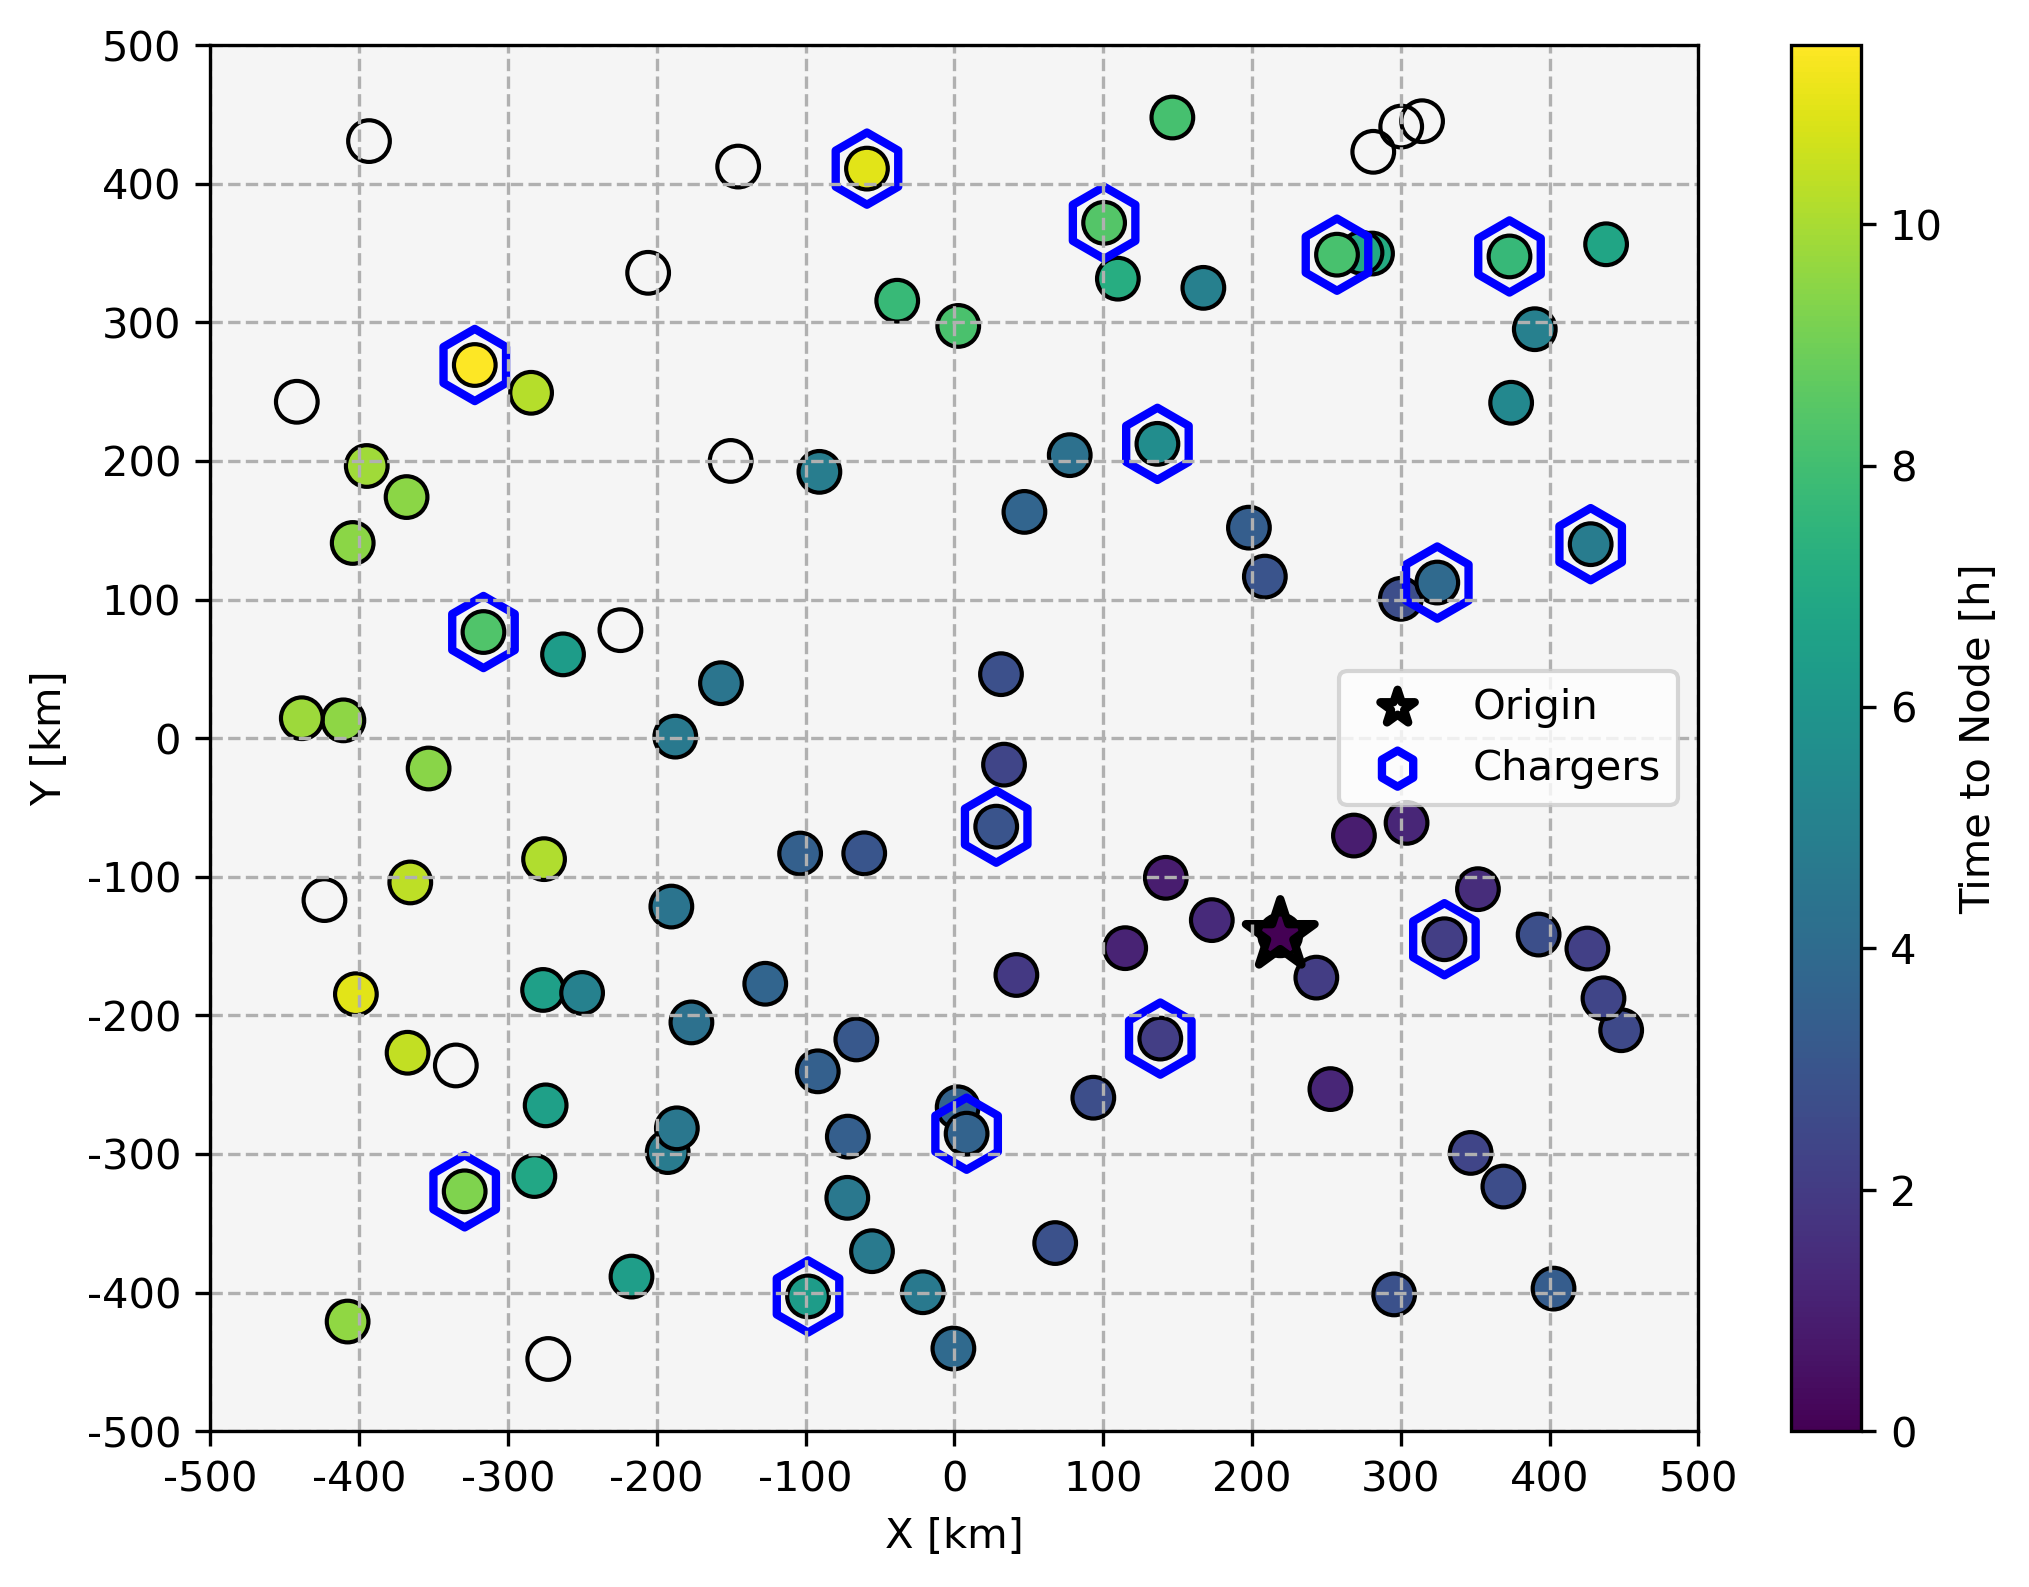
\includegraphics[width = \linewidth]{figs/interactions_la.png}
	%		\captionsetup{width=.8\linewidth}
	%		\caption{Low charger usability and aggressive risk attitude}
	%	\end{subfigure}%
%	\begin{subfigure}{.4\linewidth}
	%		\centering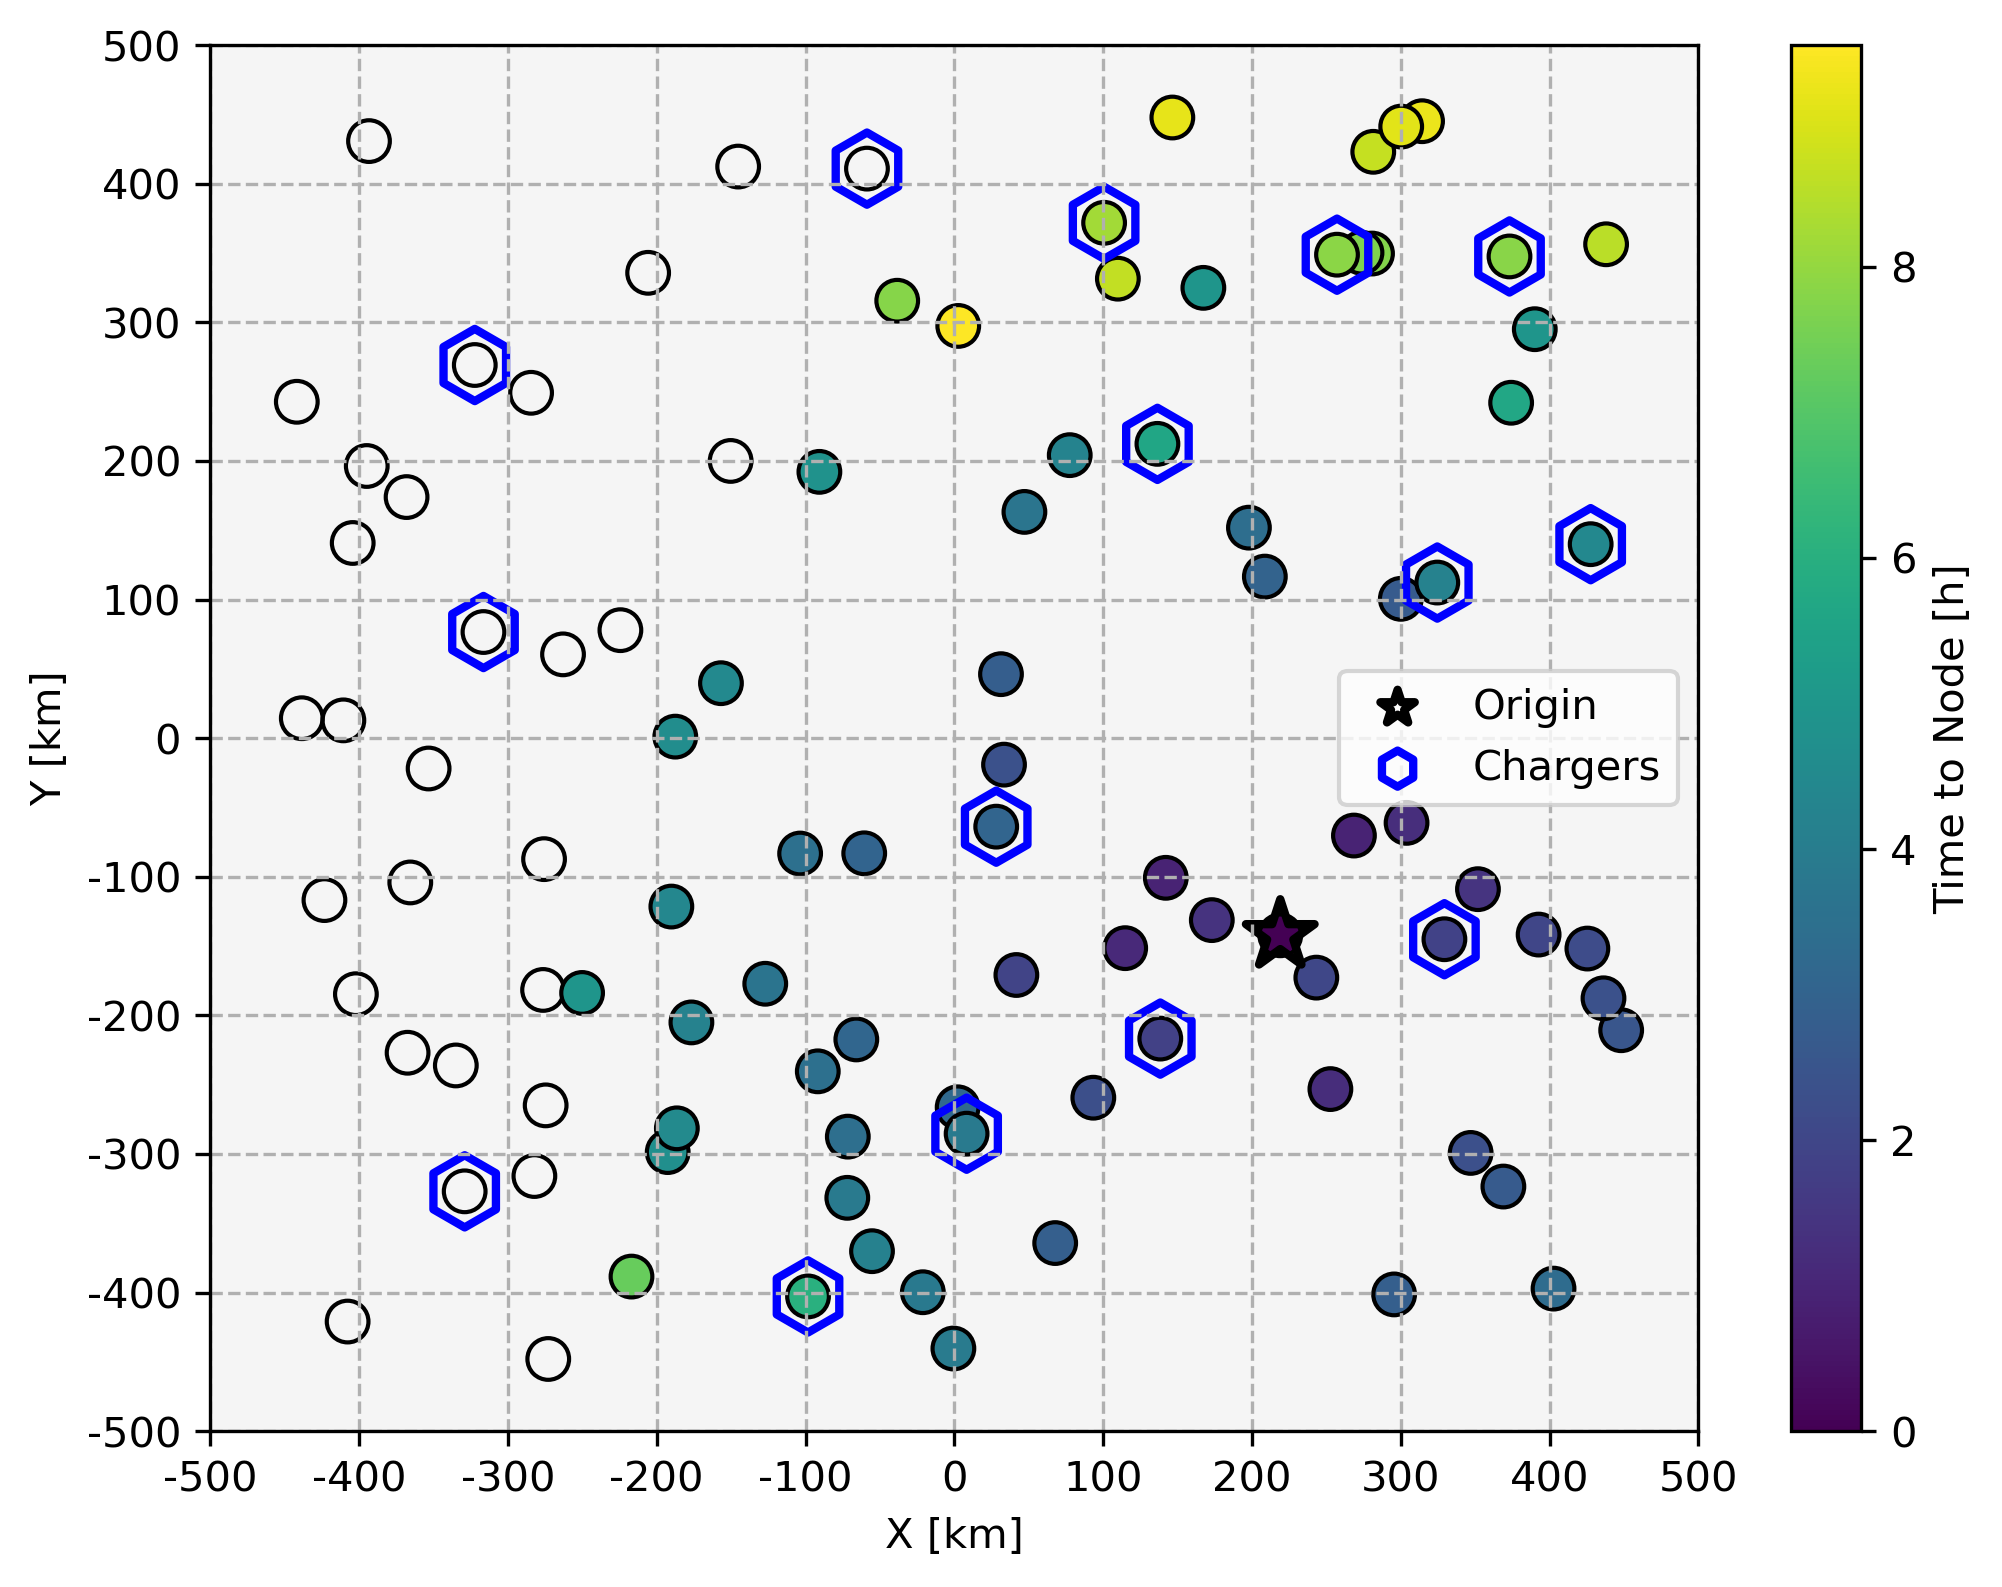
\includegraphics[width = \linewidth]{figs/interactions_lc.png}
	%		\captionsetup{width=.8\linewidth}
	%		\caption{Low charger usability and cautious risk attitude}
	%	\end{subfigure}
%	\caption{Single-origin expected travel time trees with varying charger reliability and driver risk tolerance}
%	\label{fig:interactions}
%\end{figure}
%
%\begin{multicols}{2}
%
%As the example shows, it is possible for the impact of several factors to be additive when made disadvantageous simultaneously. Where the driver has an aggressive risk attitude, chargers are reliable, or both, accessibility is high. Where neither is the case accessibility is low. The differential can be dramatic and this highlights the importance of considering vehicular, infrastructural, and behavioral factors simultaneously to get a complete picture.